\documentclass{report}

% Import necessary packages
\usepackage{amsmath}
\usepackage{array}
\usepackage[hyphens]{url}
\usepackage{amssymb}
\usepackage{multicol}
\usepackage{pgfplots}
\usepackage{empheq}
\usetikzlibrary{mindmap,trees}
\usepackage{tkz-tab}
\usepackage{tikz}
\usepackage{tcolorbox}
\usepackage{interval}
\usepackage{enumitem, pifont}
\usepackage{yhmath}
\usetikzlibrary{trees}
\usetikzlibrary{arrows.meta}  
\usepackage[pdfauthor={{Peter.C}}, pdftitle={{Mathématiques 1ere}}, pdfstartview=Fit, pdfpagelayout=SinglePage, pdfnewwindow=true, bookmarksnumbered=true, breaklinks, colorlinks, linkcolor=black, urlcolor=black, citecolor=cyan, linktoc=all]{hyperref}

% Document margins
\usepackage[margin=4cm,top=3cm, bottom=2.5cm,heightrounded]{geometry}

\usepackage{mathtools, stmaryrd}
\usepackage{xparse} \DeclarePairedDelimiterX{\Iintv}[1]{\llbracket}{\rrbracket}{\iintvargs{#1}}
\NewDocumentCommand{\iintvargs}{>{\SplitArgument{1}{,}}m}
{\iintvargsaux#1} %
\NewDocumentCommand{\iintvargsaux}{mm} {#1\mkern1.5mu..\mkern1.5mu#2}

\hypersetup{hidelinks}
\newcolumntype{C}[1]{>{\centering\arraybackslash}m{#1}}
\renewcommand{\baselinestretch}{1}
\pgfplotsset{compat=1.18}

\setcounter{tocdepth}{1}

\setlength{\parindent}{0pt}
\setlength{\parskip}{0.0em}

\definecolor{darkred}{RGB}{139,0,0}
\definecolor{darkgreen}{RGB}{0,100,0}

% Configure section numbering
\renewcommand{\thesection}{\arabic{section}} % Use integer numbering
\renewcommand{\thesubsection}{\thesection.\arabic{subsection}} % Ensure subsections follow section numbering

\newcommand{\defi}{\subsubsection{\textcolor{darkred}{Def}}}
\newcommand{\prop}{\subsubsection{\textcolor{darkgreen}{Prop}}}

\newcommand{\ptn}{\forall n \in \mathbb{N},}

\newcommand{\un}{$(u_n)$~}
\newcommand{\vn}{$(v_n)$~}
\newcommand{\pc}{+ \mathcal{C}}

\newcommand{\R}{\mathbb{R}}
\newcommand{\N}{\mathbb{N}}
\newcommand{\Z}{\mathbb{Z}}

\newcommand{\bigEps}{\mathcal{E}}
\newcommand{\vu}{\overrightarrow{u}}
\newcommand{\vv}{\overrightarrow{v}}
\newcommand{\uv}{\overrightarrow{u} \cdot \overrightarrow{v}}
\newcommand{\Cf}{\mathcal{C}_f}
\newcommand{\Sys}{(S)}

\newcommand{\gpe}{\mathrel{\rotatebox[origin=c]{30}{$=$}\mkern-3mu>}}

\newcommand{\eq}{\Leftrightarrow}

\newcommand{\air}{\vspace{1em}}

\newcommand{\ppcm}{\operatorname{ppcm}}
\newcommand{\pgcd}{\operatorname{pgcd}}

\newcommand{\qvq}{\quad , \quad}



\begin{document}


    \begin{titlepage}
        \centering
        \vspace*{2cm}
        %\includegraphics[width=0.4\textwidth]{logo_universite.png}\par\vspace{1cm}
        {\scshape\Large Lycée Louis de Broglie \par}
        {\scshape\Large \& \par}
        {\scshape\Large PTSI Jean-Baptiste Say \par}
        \vspace{1cm}
        {\scshape\Large 2023-2026 \par}
        \vspace{1.5cm}
        {\huge\bfseries Cours de Mathématiques \\ 1ère, Tale (Expert), PTSI sup\par}
        \vspace{2cm}
        {\Large\itshape Par Peter.C\par}
        \vfill
        {\large Cours et exos sur \url{https://pi-t-maths.netlify.app}\par}

    \end{titlepage}





  \newpage

    \renewcommand{\contentsname}{Sommaire}
    \tableofcontents

  \newpage

  \part{Lycée - Spécialité}
  
    \setcounter{section}{0}

    \section{Suites Numériques}

    \subsection{Généralités}

    Les suites numériques sont des listes ordonnées d'éléments numériques, des applications sur $\mathbb{R}$ d'un entier naturel ; ainsi $n \mapsto u_n : \mathbb{N} \mapsto \mathbb{R}$. On les note généralement $(u_n)$ où $n$ est l'indice du terme.

    \subsection{Suites Arithmétiques}

      Une suite arithmétique a une différence constante entre ses termes successifs.

    \subsubsection*{Sens de Variation :}

      \begin{itemize}
        \item $r > 0$, $u$ croissante, 
        \item $r = 0$, $u$ constante,
        \item $r < 0$, $u$ décroissante
      \end{itemize} 


    \subsection{Suites Géométriques}

    Une suite géométrique a un rapport constant entre ses termes successifs.

    \subsubsection{Sens de Variation :} 
      \begin{itemize}
        \item $q > 1$, ~~~~~~~~~~~~~~~$u$ croissante si $u_0 > 0$, décroissante sinon, 
        \item $1 > q > 0$,~~~~~~~~~~ $u$ décroissante si $u_0 > 0$, croissante sinon,
        \item $q = 0$ ou $u_0 = 0$, ~~$u$ constante égale à 0
      \end{itemize} 

    % Tableau récapitulatif

    \subsection{Formules}

    \begin{table}[htp!]
        \centering
        \renewcommand{\arraystretch}{2} % Ajuste la hauteur des lignes
        \begin{tabular*}{\textwidth}{| @{\extracolsep{\fill}} |c|c|c|}
            \hline
            & \textbf{Suite Arithmétique} & \textbf{Suite Géométrique} \\
            \hline
            \textbf{Récurrence} & $\displaystyle u_{n+1} = u_n + r$ & $\displaystyle u_{n+1} = u_n \times q$ \\
            \hline
            \textbf{Forme Explicite} & $\displaystyle u_n = u_p + (n-p)r$ & $\displaystyle u_n = u_p \times q^{n-p}$ \\
            \hline
            \textbf{Somme des Termes} & $\displaystyle S_n = (n-p+1)\times \frac{(u_n+u_p)}{2}$ & $\displaystyle S_n = u_p \times \frac{1 - q^{n-p+1} }{1 - q}$ \\
            \hline
            \textbf{Calculs de Nombres} & $\displaystyle 1+...+n = \frac{n(n+1)}{2}$ & $\displaystyle 1 \times ... \times n = \frac{1-q^{n-p+1}}{1-q}$ \\
            \hline
        \end{tabular*}
        \caption{Récapitulatif des Formules sur les Suites Numériques}
        \label{tab:suites}
    \end{table}

    Avec $S_n = \displaystyle\sum_{k=p}^{n} u_k = u_p + u_{p+1} + ... + u_{n-1}+ u_n$

    \subsection{Déterminer le sens de variation}

    \begin{itemize}
      \item étudier le signe de $\displaystyle u_{n+1}-u_n$
      \item étudier le signe de $\displaystyle \frac{u_{n+1}}{u_n} - 1$
      \item étudier les variations de $f$ telle que $u_n = f(n)$
      \item conjecturer et démontrer par récurence
    \end{itemize}

    %\newpage

    \subsection{Limites de suites}

    \paragraph{Définition}
    On dit qu'une suite $(u_n)$ converge vers une limite réelle $l$ lorsque $n \to +\infty$ ssi tout intervalle ouvert contenant $l$ contient tout les termes de la suite à partir d'un certain rang. Formellement : 

    \[\forall (a,b)\in(\mathbb{R}_*^+)^2, ~~ \exists N\in\mathbb{N}, ~~\forall n \geq N ~~ u_n \in ]l-a,l+b[\]

    On note alors :
    \[
    \lim_{n \to +\infty} u_n = l
    \]

    Si la suite diverge vers un infini, la suite aura tout ses termes supérieures (resp. inferieurs) à tout réel A à partir d'un certain rang. On note alors :
    \[
    \lim_{n \to +\infty} u_n = \pm \infty
    \]

    \subsubsection{Def Suite Monotone}

    On dit qu'une suite \un est monotone sur $I$ ssi elle est croissante ou décroissante sur cet intervalle.

    \subsubsection{Def Suite Minorée/Majorée}

    \begin{itemize}
      \item \textbf{$m$ minore \un} $\Rightarrow \forall n \in I ~~ u_n \geq m$
      \item \textbf{$M$ majore \un} $\Rightarrow \forall n \in I ~~ u_n \le M$
    \end{itemize}

    \subsubsection{Théorème des Suites Monotones}

    Si une suite $(u_n)$ est croissante et majorée ou décroissante et minorée, alors elle converge.

    \subsubsection{Justification de la limite d'une suite définie par récurrence}

    On a donc \un croissante (resp. décroissante) et majorée (resp. minorée), donc elle converge vers un réel $l$. On note que $u_{n+1} = f(u_n)$.

    \begin{align*}
      &\boxed{\lim_{n\to+\infty} u_n = l \Rightarrow \lim_{n\to+\infty} u_{n+1} = l} \\
      \text{donc~} &\boxed{\lim_{n\to+\infty} u_{n+1} = \lim_{n\to+\infty} f(u_n) = f(l) = l } ~\textbf{par unicité de la limite}\\
      \text{donc~} &\boxed{~l = f(l) \Leftrightarrow \cdots \Leftrightarrow l = a} \\
      \text{donc~} &\boxed{\lim_{n\to+\infty} u_n = a}
    \end{align*}

    \subsubsection{Limites usuelles et opérations sur les limites}

    Voir \nameref{sec:limFonction}

    \iffalse
    Soient $(u_n)$ et $(v_n)$ deux suites avec $\lim_{n \to +\infty} u_n = l$ et $\lim_{n \to +\infty} v_n = m$. Alors :
    \begin{itemize}
        \item $\lim_{n \to +\infty} (u_n + v_n) = l + m$
        \item $\lim_{n \to +\infty} (u_n \cdot v_n) = l \cdot m$
        \item Si $m \neq 0$, $\lim_{n \to +\infty} \frac{u_n}{v_n} = \frac{l}{m}$
    \end{itemize}
    \fi

    \iffalse
    \subsection{Exemples de Suites Divergentes}
    - Suite géométrique de raison supérieure à 1 : $(u_n) = 2^n \to +\infty$ quand $n \to +\infty$.
    - Suite harmonique $(u_n) = \frac{1}{n}$ : $\lim_{n \to +\infty} u_n = 0$ (convergence vers 0).
    \fi



    \newpage


    \section{Probabilités}
    \subsection{Généralités}

    \paragraph{Définitions}

    \begin{itemize}
        \item \textbf{Univers $\Omega$} : Ensemble de tous les résultats possibles d'une expérience aléatoire.
        \item \textbf{Événement} : Sous-ensemble de l'univers $\Omega$.
        \item \textbf{Probabilité} : Fonction $P$ qui assigne à chaque événement $A$ une valeur $P(A)$, telle que pour tout événement $A$ :
        \begin{enumerate}
            \item $0 \leq P(A) \leq 1$
            \item $P(\Omega) = 1$
            \item $P(\bar{A}) = 1 - P(A)$ , $\bar{A}$ est appelé \textit{événement contraire de $A$}
        \end{enumerate}
        \item \textbf{Vocabulaire}
        \begin{itemize}
          \item \textbf{disjonction de A et B} $= A \cup B$
          \item \textbf{conjonction de A et B} $= A \cap B$
        \end{itemize}
    \end{itemize}

    \paragraph{Formules Importantes}

    \begin{itemize}
        \item \textbf{Probabilité de l'union}
        \[P(A \cup B) = P(A) + P(B) - P(A \cap B)\]
        \item \textbf{Evènements incompatibles}
        \[P(A \cap B) = 0 \Rightarrow \text{"A ; B \textbf{incompatibles}"}\]
        \item \textbf{Probabilités Conditionnelles}
        \[P(A \cap B) = P_B(A) \cdot P(B) = P_A(B) \cdot P(A)\]
        \item \textbf{Probabilités Totales}
        \[P(B) = \sum_{k=1}^{n} P(A_k) \cdot P_{A_k}(B) = \sum_{k=1}^{n}P(A_k \cap B)\]
        
    \end{itemize}

    \subsection{Arbre de probabilité}
    \centering
    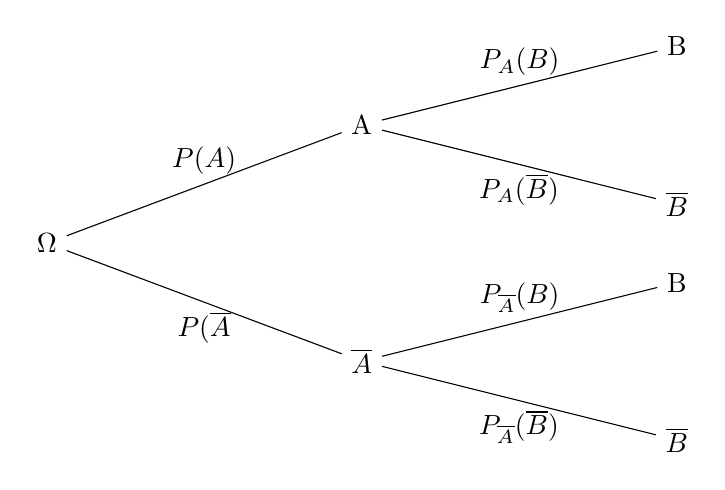
\begin{tikzpicture}
        [
          grow=right,
          level distance=4cm,
          level 1/.style={sibling distance=3cm},
          level 2/.style={sibling distance=2cm},
          level 3/.style={sibling distance=1cm},
          edge from parent/.style={draw},
          every node/.style={align=center}
        ]
        
        \node {$\Omega$}
          child {
            node {$\overline{A}$}
            child {
              node {$\overline{B}$}
              edge from parent node[below] {$P_{\overline{A}}(\overline{B})$}
            }
            child {
              node {$\text{B}$}
              edge from parent node[above] {$P_{\overline{A}}(B)$}
            }
            edge from parent node[below] {$P(\overline{A}$}
          }
          child {
            node {A}
            child {
              node {$\overline{B}$}
              edge from parent node[below] {$P_{A}(\overline{B})$}
            }
            child {
              node {B}
              edge from parent node[above] {$P_A(B)$}
            }
            edge from parent node[above] {$P(A)$}
          };
    \end{tikzpicture}
    \raggedright

    \newpage

    \subsection{Probabilités Indépendantes}

      \paragraph{Definition}
      Deux événements $A$ et $B$ sont indépendants si et seulement si :
      \[P_B(A) = P(A)\]
      %\[P(A \cap B) = P_B(A) \cdot P(A)\]

      \paragraph{Corrollaires}

      Si $A$ et $B$ sont indépendants, alors :
      \begin{itemize}
          \item $P_B(A) = P(A)$ et $P_A(B) = P(B)$
          \item $P(A \cap B) = P(B) \cdot P(A)$
          \item Si $A_1, A_2, \ldots, A_n$ sont des événements mutuellement indépendants, alors :
          \[P(A_1 \cap A_2 \cap \ldots \cap A_n) = \prod_{k=1}^{n} P(A_k)\]
          ce qui représente la propabilité de l'évènement présent au bout du chemin $A_1, A_2, \ldots, A_n$
          \item $A$ et $B$ indépendants $\Rightarrow$ $\overline{A}$ et $B$ indépendants    
      \end{itemize}

    \subsection{Variable aléatoire}

    \paragraph{Définition}
    X est une variable aléatoire en tant qu'application de $\Omega$ dans $\mathbb{R}$

    \paragraph{Loi de probabilité} ~\\ ~

    \begin{table}[htp!]
      \begin{center}
        \begin{tabular}{|c|c|c|c|c|}
          \hline
          Valeur de $x_i$ & $x_1$ & $x_2$ & $\ldots$  & $x_n$ \\ \hline
          Proba $P(X=x_i)$ & $p_1$ & $p_2$ & $\ldots$ & $p_n$ \\ \hline
        \end{tabular}
      \end{center}
    \end{table}

    \paragraph{Espérance et Variance}
    \begin{align*}
      E(X) &= \sum_{i=1}^{n} p_i x_i \\
      V(X) &= \sum_{i=1}^{n} p_i (x_i - E(X))^2
    \end{align*}

    \paragraph{Ecart-type}

    \[\sigma(X) = \sqrt{V(X)}\]

    \paragraph{Loi binomiale}
    Dans le cas d'une répétition de $n$ expériences identiques et indépendantes, on est dans le cas d'un Schéma de Bernoulli. On note : \(\boxed{Y\sim \mathcal{B}(n;p)}\)
    et : 

    \[P(Y=k) = binomFdp(k, n, p) = \binom{n}{k} p^k (1-p)^{n-k}\]

    \newpage


    \section{Équations du Second Degré}

    \subsection{Forme Générale}

    Une équation du second degré est une équation polynomiale de la forme :

    \[ ax^2 + bx + c = 0 \]

    où \( a \), \( b \) et \( c \) sont des constantes réelles avec \( a \neq 0 \).

    \subsection{Discriminant}

    Le discriminant \( \Delta \) d'une équation du second degré \( ax^2 + bx + c = 0 \) est défini comme :

    \[ \Delta = b^2 - 4ac \]

    \begin{itemize}
        \item Si \( \Delta > 0 \), l'équation a deux solutions réelles distinctes.
        \item Si \( \Delta = 0 \), l'équation a une seule solution réelle double.
        \item Si \( \Delta < 0 \), l'équation n'a pas de solution réelle.
    \end{itemize}

    \subsection{Formules de Solutions}

    Les solutions de l'équation du second degré \( ax^2 + bx + c = 0 \) sont données par :

    \[ x = \frac{-b \pm \sqrt{\Delta}}{2a} \]

    \subsection{Sommes et Produits des Racines}

    Pour une équation du second degré, les somme S et produit P des racines $x_1$ et $x_2$ sont donnés par :

    \[
    \begin{aligned}
        S = -\frac{b}{a}~~~~~
        P = \frac{c}{a}
    \end{aligned}
    \]

    \subsection{Forme Canonique}

    Une équation du second degré peut être transformée en forme canonique : \[ a(x - \alpha)^2+ \beta = 0\]

    Avec : $\alpha = \frac{-b}{2a} \quad \text{et} \quad \beta = f(\alpha)$. \\
    On obtient souvent cette forme via l'identité remarquable $a^2+2ab+b^2=(a+b)^2$


    \vfill

    \section{Identités remarquables}

    \label{IDR}

      \begin{center}
        \begin{minipage}{0.49\textwidth}
          \begin{tcolorbox}[colback=white, colframe=black, boxrule=0.5pt, width=\textwidth]
            \begin{center}
              \((a\pm b)^2 = a^2 \pm2ab + b^2\) \\
              \((a+b)(a-b) = a^2-b^2\)
            \end{center}
          \end{tcolorbox}
        \end{minipage}
        \hfill
        \begin{minipage}{0.49\textwidth}
          \begin{center}
            \begin{tcolorbox}[colback=white, colframe=black, boxrule=0.5pt, width=\textwidth]
              \((a\pm b)^3 = a^3 \pm3a^2b +3ab^2\pm b^3\) \\
              \((a\pm b)(a^2 \mp 2ab + b^2) = a^3\pm b^3\)
            \end{tcolorbox}
          \end{center}
        \end{minipage}
      \end{center}

      \begin{tcolorbox}[colback=white, colframe=black, boxrule=0.5pt, width=\textwidth]\[(a+b+c)^2 = a^2 + b^2 +c^2 +2ab+2bc+ 2ac\]\end{tcolorbox}
    

    




    \newpage





    \section{Dérivation}
    \label{deriv}

    %\subsection{Définition}

    Soit une fonction $f$ continue et dérivable sur un intervalle $I$.

    %La dérivée d'une fonction \( f(x) \), notée \( f'(x) \) ou \( \frac{df}{dx} \), représente le taux de variation instantané de \( f(x) \) par rapport à \( x \). %Géométriquement, elle correspond à la pente de la tangente au graphe de la fonction à un point donné.

    \subsection{Définitions}

     \paragraph{Taux d'accroissement}

    Le taux d'accroissement d'une fonction \( f(x) \) sur un intervalle \( [a, a+h] \) est défini comme la variation de la fonction sur cet intervalle, divisée par la variation de la variable indépendante. Formellement, le taux d'accroissement $t$ est donné par :

    \[ T(h) = \frac{f(a+h) - f(a)}{h} \]

    \paragraph{Interprétation Géométrique}

    Géométriquement, le taux d'accroissement représente la pente de la droite sécante reliant les points \( (a, f(a)) \) et \( (a+h, f(a+h)) \) sur le graphe de la fonction.

    \paragraph{Nombre dérivé}

    On note $f'(a)$ le nombre dérivé de $C_f$ au point $a$, tel que :
    \[ \forall a \in I ~ , \quad f'(a) = \lim_{h \to 0} T(h) \]

    \paragraph{Derivée seconde}

      On note $f''(x)$ la fonction dérivée seconde de $f$, tel que :
      \[ \forall x \in I ~ , \quad f''(x) = \left(f'(a)\right)' \]

    \paragraph{Convexité} Si pour tout $x$ de $I$, $f''(x)\ge 0$ alors $f$ est dite convexe sur $I$. On a alors que tout segment reliant $A$ et $B$ deux points de $\Cf$ sur $I$ est au dessus de $\Cf$ ; et toute tangeante à $\Cf$ sur $I$ est en dessous de $\Cf$. De la première propriété découle la formule suivante :

    \[\forall (x, x')\in I ~, \quad \forall \lambda \in \left[0;1\right] ~ , \quad f(\lambda x + (1 - \lambda)x') \le \lambda f(x) + (1-\lambda)f(x'   )\]

    \subsection{Dérivées de Fonctions Usuelles}

    \begin{table}[h]
      \centering
      \renewcommand{\arraystretch}{1.4} % Ajuste la hauteur des lignes
      \begin{tabular*}{\textwidth}{|@{\extracolsep{\fill}}c|c|c|c|}
          \hline
          \textbf{~~Fonction} & \textbf{\(D_f\)} & \textbf{\(D_{f'}\)} & \textbf{Fonction dérivée} \\
          \hline
          \( ax + b \) & \( \mathbb{R} \) & \( \mathbb{R} \) & \( a \) \\
          \hline
          \( x^n \) & \( \mathbb{R} \) & \( \mathbb{R} \) & \( nx^{n-1} \) \\
          \hline
          \( \dfrac{1}{x^n} \) & \( \mathbb{R}^* \) & \( \mathbb{R}^* \) & \( -\dfrac{n}{x^{n+1}} \) \\
          \hline
          \( \sqrt{x} \) & \( \mathbb{R}^*_+ \) & \( \mathbb{R}^*_+ \) & \( \dfrac{1}{2\sqrt{x}} \) \\
          \hline
          \( \sin x \) & \( \mathbb{R} \) & \( \mathbb{R} \) & \( \cos x \) \\
          \hline
          \( \cos x \) & \( \mathbb{R} \) & \( \mathbb{R} \) & \( -\sin x \) \\
          \hline
          \( \tan x \) & \( \mathbb{R}\setminus\left\{\tfrac{\pi}{2}+k\pi \mid k\in\mathbb{Z}\right\} \) & \( \mathbb{R}\setminus\left\{\tfrac{\pi}{2}+k\pi \mid k\in\mathbb{Z}\right\} \) & \( \dfrac{1}{\cos^2 x}  = 1 + \tan^2(x)\) \\
          \hline
          \( e^x \) & \( \mathbb{R} \) & \( \mathbb{R} \) & \( e^x \) \\
          \hline
          \( \ln(x) \) & \( \mathbb{R}^*_+ \) & \( \mathbb{R}^*_+ \) & \( \dfrac{1}{x} \) \\
          \hline
      \end{tabular*}
      \caption{Dérivées de fonctions usuelles}
      \label{tab:derivatives}
  \end{table}
  

    \newpage


    \subsection{Règles de Dérivation}

    Soit \( u(x) \) et \( v(x) \) deux fonctions dérivables et \( c \) une constante réelle, les règles de dérivation suivantes s'appliquent :
    \iffalse
      \begin{itemize}
        \item \textbf{Équation de $T_a$} : $f'(a)(x-a)+f(a)$
        \item \textbf{Dérivée de la somme} : \( (u + v)' = u' + v' \)
        \item \textbf{Dérivée du produit avec une constante} : \( (ku)' = ku' \)
        \item \textbf{Dérivée du produit} : \( (uv)' = u'v + uv' \)
        \item \textbf{Dérivée de l'inverse} : \(\displaystyle \left(\frac{1}{v}\right)' = \frac{-v'}{v^2} \), avec \( v \neq 0 \)
        \item \textbf{Dérivée du quotient} : \(\displaystyle \left(\frac{u}{v}\right)' = \frac{u'v - uv'}{v^2} \), avec \( v \neq 0 \)
        \item \textbf{Dérivée de la fonction composée} : \(\displaystyle (f(g(x)))' = f'(g(x)) \cdot g'(x) \)
        \item \textbf{Dérivée de la fonction inverse} : \(\displaystyle (f^{-1})'(x) = \frac{1}{f'(f^{-1}(x))} \)
        \item \textbf{Dérivée de la fonction exponentielle} : \( (e^{u})' = u' e^{u} \)
        \item \textbf{Dérivée de la fonction logarithme népérien} : \( (\ln(x))' = \frac{1}{x} \)
      \end{itemize}


      \begin{table}[h]
        \centering
        \renewcommand{\arraystretch}{1.7} % Ajuste la hauteur des lignes
        \begin{tabular}{|l|c|c|}
          \hline
          \textbf{Dérivée de ...} & \textbf{f(x)} & \textbf{f'(x)} \\
          \hline
          \textbf{Somme} & \( \displaystyle u + v \) & \( \displaystyle u' + v' \) \\
          \hline
          \textbf{Produit avec une constante} & \( \displaystyle ku \) & \( \displaystyle ku' \) \\
          \hline
          \textbf{Produit} & \( \displaystyle uv \) & \( \displaystyle u'v + uv' \) \\
          \hline
          \textbf{Inverse} & \( \displaystyle \frac{1}{v} \) & \( \displaystyle \frac{-v'}{v^2} \), avec \( v \neq 0 \) \\
          \hline
          \textbf{Quotient} & \( \displaystyle \frac{u}{v} \) & \( \displaystyle \frac{u'v - uv'}{v^2} \), avec \( v \neq 0 \) \\
          \hline
          \textbf{Fonction composée} & \( \displaystyle f(g(x)) \) & \( \displaystyle f'(g(x)) \cdot g'(x) \) \\
          \hline
          \textbf{Fonction inverse} & \( \displaystyle f^{-1}(x) \) & \( \displaystyle \frac{1}{f'(f^{-1}(x))} \) \\
          \hline
          \textbf{Fonction exponentielle} & \( \displaystyle e^u \) & \( \displaystyle u' e^u \) \\
          \hline
          \textbf{Fonction logarithme népérien} & \( \displaystyle \ln(x) \) & \( \displaystyle \frac{1}{x} \) \\
          \hline
        \end{tabular}
      \end{table}
    \fi

    \begin{table}[h]
      \centering
      \renewcommand{\arraystretch}{1.7}
      \begin{tabular}{|>{\centering\arraybackslash}p{6cm}|>{\centering\arraybackslash}p{6cm}|}
        \hline
        \textbf{f(x)} & \textbf{f'(x)} \\
        \hline
        \( \displaystyle u + v \) & \( \displaystyle u' + v' \) \\
        \hline
        \( \displaystyle ku \) & \( \displaystyle ku' \) \\
        \hline
        \( \displaystyle uv \) & \( \displaystyle u'v + uv' \) \\
        \hline
        \( \displaystyle \frac{1}{v} \) & \( \displaystyle \frac{-v'}{v^2} \), avec \( v \neq 0 \) \\
        \hline
        \( \displaystyle \frac{u}{v} \) & \( \displaystyle \frac{u'v - uv'}{v^2} \), avec \( v \neq 0 \) \\
        \hline
        \( \displaystyle f \circ g(x) = f(g(x))\) & \( \displaystyle f'(g(x)) \cdot g'(x) \) \\
        %\hline
        %\( \displaystyle f^{-1}(x) \) & \( \displaystyle \frac{1}{f'(f^{-1}(x))} \) \\
        %\hline
        %\( \displaystyle e^u \) & \( \displaystyle u' e^u \) \\
        %\hline
        %\( \displaystyle \ln(u) \) & \( \displaystyle \frac{u'}{u} \) \\
        \hline
      \end{tabular}
    \end{table}


    \subsection{Application de la Dérivée}

    Pour étudier les variations de la fonction \( f(x) \), on peut utiliser le signe de sa dérivée \( f'(x) \). Voici un tableau de variation typique (polynome 2nd degré) :

    \begin{center}
      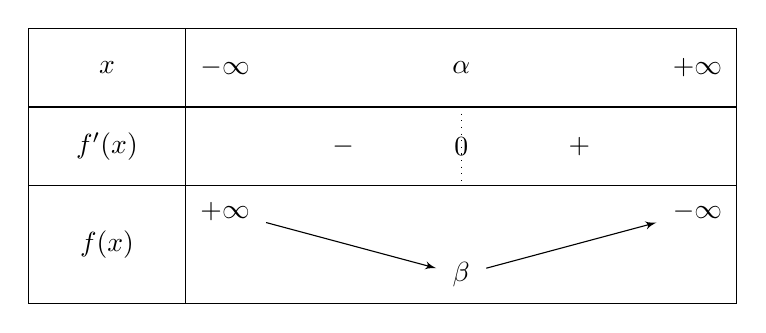
\begin{tikzpicture}
        \tkzTabInit{$x$ / 1 , $f'(x)$ / 1, $f(x)$ / 1.5}{$-\infty$, $\alpha$, $+\infty$}
        \tkzTabLine{, -, z, +, }
        \tkzTabVar{+/ $+\infty$, -/ $\beta$, +/ $-\infty$}
      \end{tikzpicture}
    \end{center}

    \subsection{Application de la Dérivée seconde}

    Pour étudier la connvexité de la fonction \( f(x) \), on peut utiliser le signe de sa dérivée seconde \( f''(x) \). Voici un tableau de connvexité typique (polynome 3eme degré) :

    \begin{center}
      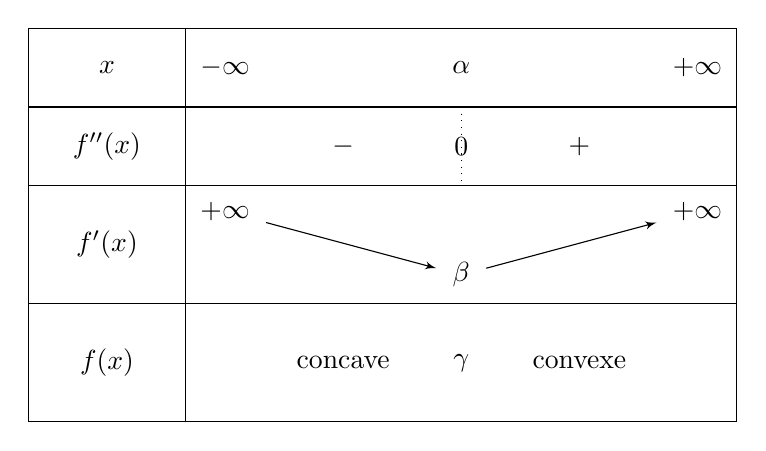
\begin{tikzpicture}
        \tkzTabInit{$x$ / 1 , $f''(x)$ / 1, $f'(x)$ / 1.5, $f(x)$ / 1.5}{$-\infty$, $\alpha$, $+\infty$}
        \tkzTabLine{ , -, z, +, }
        \tkzTabVar{+/ $+\infty$, -/ $\beta$, +/ $+\infty$}
        \tkzTabLine{ , \text{concave}, \gamma, \text{convexe}, }
      \end{tikzpicture}
    \end{center}

    \newpage

    \section{Fonction exponentielle}
    \subsection{Définition}
    On défini la fonction $exp(x)$ l'unique fonction dérivable sur $\mathbb{R}$ tel que $\forall x \in \mathbb{R}$ : \[exp'(x) = exp(x) ~~~~et~~~~ exp(0)=1\]

    \paragraph{Note} Voir \nameref{deriv} pour les rêgles de dérivation de la fonction.

    \subsection{Rêgles de calcul}
    Pour gagner du temps en expliquations rébarbatives, on assimilera la fonction $exp(x)$ à $e^x$ où $e \approx 2,71828$, et par conséquent toutes les rêgles de calcul sur la fonction exponentielle correspondent à celles des puissances. 
    Ainsi $\forall (x,y) \in \mathbb{R}^2$, $\forall k \in \mathbb{Z}$ : 
    \[e^0=1 ~~~~et~~~~ e^1=e\]
    \[e^{x+y}=e^{x}*e^{y}\]
    \[e^{x-y}=e^{x} / e^{y}\]
    \[e^{-x}=\frac{1}{e^x}\]
    \[e^{kx}=(e^{x})^k\]

    On note que e étant positif, $e^x > 0 , \forall x \in \mathbb{R}$ et exp strictement croissante sur $\mathbb{R}$ ou $exp : \mathbb{R} \rightarrow \mathbb{R}^{+*}$

    \[\forall (x,y) \in \mathbb{R}, x < y \Leftrightarrow e^x < e^y\]

    \subsection{Représentation graphique}

    \begin{center}
      \begin{tikzpicture}[>=stealth]
        \begin{axis}[
            xmin=-4,xmax=4,
            ymin=-2,ymax=6,
            axis x line=middle,
            axis y line=middle,
            axis line style=->,
            xlabel={$x$},
            ylabel={$y$},
            xtick={-4,-3,-2,-1,0,1,2,3,4},
            xticklabels={$-4$,$-3$,$-2$,$-1$,$0$,$1$,$2$,$3$,$4$},
            ytick={-2,-1,0,1,2,3,4,5,6},
            yticklabels={$-2$,$-1$,$0$,$1$,$2$,$3$,$4$,$5$,$6$},
            ]
            \addplot[no marks,blue,] expression[domain=-4.1:4,samples=100]{e^x} 
                        node[pos=0.65,anchor=south west]{$y=e^x$}; 
        \end{axis}
    \end{tikzpicture}
    \end{center}

    \subsection{Equations}
    On nottera la formule permettant de résoudre la majeure partie des equations contenant des exponentielles : 
    \[e^a = e^b \Leftrightarrow a = b ~~~ avec~a~et~b~dans~\mathbb{R}\]

    \newpage



    \section{Fonction logarithme népérien}

    \subsection{Définition}

    La fonction logarithme népérien, notée \(\ln(x)\), est la \textbf{fonction réciproque} de la fonction exponentielle \(e^x\). Elle est définie pour tout \(x > 0\)  et est solution de l'équation \(e^y = x\). Autrement dit :
    \[
    \forall x \in \mathbb{R}^*_+ ~,~~ \boxed{\ln(x) = y \iff e^y = x}
    \]

    %Pour tout réel \(y > 0\), l'équation \(e^x = y\) admet une unique solution \(x = \ln(y)\). La fonction logarithme népérien est donc définie sur \([0, +\infty[\) et associe à tout réel \(y > 0\) l'unique solution de l'équation \(e^x = y\), notée \(\ln(y)\).

    \subsection{Propriétés}

    \begin{itemize}
        \item \textbf{Domaines :} $D_{ln} = ]0; +\infty[$
        \item \textbf{Accroissement :} $ln$ est strictement croissante sur $D_{ln}$.
        \item \textbf{Limites :} \(\boxed{\lim_{\substack{x\to 0 \\ >}} ~~~\ln(x) = -\infty}\) et \(\boxed{\lim_{x \to +\infty} \ln(x) = +\infty}\)

    \end{itemize}

    \iffalse\subsection{Dérivée}

    \[
    \forall x \in \mathbb{R}^*_+ , \boxed{\quad \ln'(x) = \frac{1}{x}}
    \]\fi

    \subsection{Propriétés Logarithmiques}

    \begin{itemize}
        \item \(\boxed{\ln(xy) = \ln(x) + \ln(y)}\) et donc \(\boxed{\ln(x^k) = k \ln(x)}\) et donc \(\boxed{\ln(\sqrt{x}) = \frac{1}{2}\ln(x)}\)
        \item \(\boxed{\displaystyle \ln\left(\frac{x}{y}\right) = \ln(x) - \ln(y)}\) et donc \(\boxed{\ln\left(\frac{1}{x}\right) = -\ln(x)}\)
    \end{itemize}

    \subsection{Représentation Graphique}

    \begin{center}
      \begin{tikzpicture}[>=stealth]
        \begin{axis}[
            xmin=0, xmax=4,
            ymin=-2, ymax=2,
            axis x line=middle,
            axis y line=middle,
            axis line style=->,
            xlabel={$x$},
            ylabel={$y$},
            xtick={0.5, 1, 2, 3, 4},
            xticklabels={$0.5$, $1$, $2$, $3$, $4$},
            ytick={-2, -1, 0, 1, 2},
            yticklabels={$-2$, $-1$, $0$, $1$, $2$},
            domain=0.1:4,
            ]

            % Plot the function
            \addplot[no marks,blue] expression[domain=0.1:4,samples=100]{ln(x)} 
                        node[pos=0.75,anchor=south east]{$y = \ln(x)$}; 

            % Define e
            \pgfmathsetmacro{\e}{exp(1)}

            % Add vertical lines from the x-axis to the curve at x=e
            \addplot[blue, dashed] coordinates {({\e},0) ({\e},{ln(\e)})};

            % Add horizontal line from the y-axis to the curve at y=ln(e)
            \addplot[blue, dashed] coordinates {(0,{ln(\e)}) ({\e},{ln(\e)})};

            % Add label "e" at the x-coordinate of the vertical line's base
            \node[below] at ({\e},0) {$e$};

        \end{axis}
      \end{tikzpicture}
    \end{center}

    \subsection{Applications}

    \begin{itemize}
        %\item \textbf{Modélisation :} Le logarithme népérien est souvent utilisé dans des modèles de croissance, des calculs de rentabilité, et en analyse de données.
        \item \textbf{Propriétés de l'équation } : \(\forall x \in \mathbb{R}^*_+ ~,~~  e^{\ln(x)} = x\) ; \(\ln(e^x) = x\) ; $x^a = e^{a\ln(x)}$
        \item \textbf{Complément aux croissances comparées}, \(\displaystyle \forall x \in \mathbb{R}^*_+\) : \(\boxed{\lim_{x\to +\infty} \frac{ln(x+1)}{x} = 1}\)
        \item \textbf{Corrollaires à la monotonie} : $\boxed{\forall x \in \mathcal{D}_n ~ , \quad \ln(x) = \ln(y) \begin{array}{c} \iff \\ \ge \end{array} x = y}$
    \end{itemize}

    \newpage

    \section{Autres fonctions usuelles}

      \subsection{Fonction partie entère}

        Soit $x$ un réel, on appelle partie entière de $x$ l'entier relatif $E(x)$ ou $\lfloor x \rfloor$, tel que : 
        \[\boxed{E(x) \le x < E(x) +1}\]

        La fonction partie entière est définie sur $\R$ par : $x \to E(x)$

        \subsubsection*{Exemples}

        \begin{align}
          E(~~4.1) &= 4\\
          E(-4.1) &= 5
        \end{align}

      \subsection{Fonction logarithme décimal}

        La fonction \textbf{logarithme décimal} est la fonction, notée \textbf{log}, définie sur $\R^*_+$, telle que :
        \[\log(x) = \frac{\ln(x)}{\ln(10)}\]
        La fonction logarithme décimal est continue, dérivable, et strictement croissante sur $\R^*_+$, et possède les mêmes propriétés algébriques que la fonction ln. Enfin, pour tout $n$ de $\mathbb{N}$ : 
        \[\log(10^p) = p\]

    \newpage


    \section{Trigonométrie}

    \subsection{Le Cercle Trigonométrique}

    Il consiste en un cercle de rayon $1$ centré à l'origine du plan cartésien. Les mesures d'angles se font ici en radians (fonctionne aussi en degrés). Voici une représentation du cercle trigonométrique :

    \begin{center}
      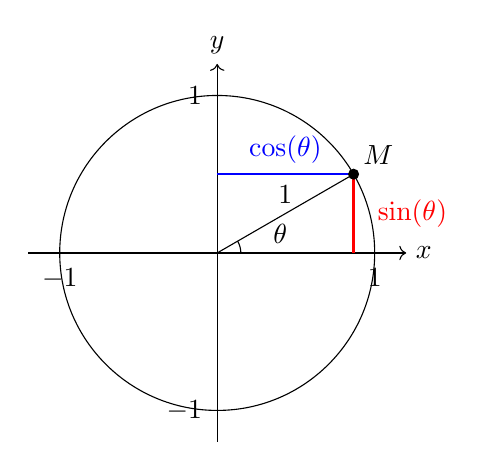
\begin{tikzpicture}[scale=2]
          \draw (0,0) circle (1);
          \draw[->] (-1.2,0) -- (1.2,0) node[right] {$x$};
          \draw[->] (0,-1.2) -- (0,1.2) node[above] {$y$};
          \foreach \x/\xtext in {-1, 1}
              \draw (\x cm,1pt) -- (\x cm,-1pt) node[anchor=north] {$\xtext$};
          \foreach \y/\ytext in {-1, 1}
              \draw (1pt,\y cm) -- (-1pt,\y cm) node[anchor=east] {$\ytext$};
          \draw (0,0) -- (30:1cm) node[midway,above] {$1$};
          \draw (0.15,0) arc (0:30:0.15cm);
          \node at (0.4,0.12) {$\theta$};
          
          % Ajout des lignes pour sin et cos
          \draw[red, thick] (30:1cm) -- (30:1cm |- 0,0) node[midway,right=5pt] {$\sin(\theta)$};
          \draw[blue, thick] (30:1cm) -- (30:1cm -| 0,0) node[midway,above] {$\cos(\theta)$};
          
          % Ajout du point M
          \fill (30:1cm) circle[radius=1pt] node[above right] {$M$};
      \end{tikzpicture}
    \end{center}

    \subsection{Le Sinus et le Cosinus}

      \begin{table}[htbp]
        \centering
        \renewcommand{\arraystretch}{2.1}
        \begin{tabular}{|>{\centering\arraybackslash}p{3cm}|*{5}{>{\centering\arraybackslash}p{2cm}|}}
          \hline
          $\theta$ (rad) & $0$ & $\displaystyle\frac{\pi}{6}$ & $\displaystyle\frac{\pi}{4}$ & $\displaystyle\frac{\pi}{3}$ & $\displaystyle\frac{\pi}{2}$ \\
          \hline
          $\theta$°& $0^\circ$ & $30^\circ$ & $45^\circ$ & $60^\circ$ & $90^\circ$ \\
          \hline
          $\sin(\theta)$ & $0$ & $\displaystyle\frac{1}{2}$ & $\displaystyle\frac{\sqrt{2}}{2}$ & $\displaystyle\frac{\sqrt{3}}{2}$ & $1$ \\
          $\cos(\theta)$ & $1$ & $\displaystyle\frac{\sqrt{3}}{2}$ & $\displaystyle\frac{\sqrt{2}}{2}$ & $\displaystyle\frac{1}{2}$ & $0$ \\
          $\tan(\theta)$ & $0$ & $\displaystyle\frac{\sqrt{3}}{3}$ & $1$ & $\displaystyle\sqrt{3}$ & $||$ \\
          \hline
        \end{tabular}
      \end{table}

      %\newpage

      \subsection{Formules fondamentales de trigonométrie}

        \paragraph{1. Formule fondamentale}
        \[
        \cos^2(x) + \sin^2(x) = 1 = ||\vec{OM}||^2
        \]

        \iffalse\paragraph{2. Formules de dérivées}
        \[
        \sin'(x) = \cos(x)
        \qquad
        \cos'(x)= -\sin(x)
        \]\fi

        \iffalse\paragraph{2. Limites usuelles}
        \[
        \lim_{x \to 0} \frac{\sin(x)}{x} = 1
        \qquad
        \lim_{x \to 0} \frac{\tan(x)}{x} = 1
        \qquad
        \lim_{x \to 0} \frac{1 - \cos(x)}{x} = 0
        \]\fi

        \paragraph{2. Formules d'addition}
        \[
        \cos(a \pm b) = \cos(a)\cos(b) \mp \sin(a)\sin(b)
        \]
        \[
        \sin(a \pm b) = \sin(a)\cos(b) \pm \cos(a)\sin(b)
        \]

        \paragraph{3. Formules de duplication}
        \begin{itemize}
          \item Pour calculer $\cos(2x)$ et $\sin(2x)$, utiliser les formules d'addition, et 
          \item \begin{align*}
                  \cos(2x) &= \cos^2(x) - \sin^2(x) = 1 - 2\sin^2(x) = 2\cos^2(x)-1 \\
                  \sin(2x) &= 2\sin(x)\cos(x) 
                \end{align*}
        \end{itemize}

        \paragraph{4. Formules de linéarisation}
        Pour linéariser ($\Sigma\to\Pi$), on trouve par addition : 
        \begin{align*}
          \cos a \cos b &= \frac{1}{2} \left(\cos(a+b)+ \cos(a-b)\right)\\
          \sin a \sin b &= \frac{1}{2} \left(\cos(a-b)- \cos(a+b)\right)\\
          \sin a \cos b &= \frac{1}{2} \left(\sin(a+b)+ \sin(a-b)\right)\\
        \end{align*}

        \paragraph{5. Formules de dé-linéarisation}
        Pour délinéariser ($\Pi\to\Sigma$), on trouve par linéar° : 
        \begin{align*}
          \cos p +\cos q &= 2 \cos(\frac{p+q}{2})\cos(\frac{p-q}{2})\\
          \cos p -\cos q &= 2 \sin(\frac{p+q}{2})\sin(\frac{p-q}{2})\\
          \sin p +\sin q &= 2 \sin(\frac{p+q}{2})\cos(\frac{p-q}{2})\\
        \end{align*}

        \iffalse\paragraph{4. Valeurs remarquables}
        \[
        \cos\left( \frac{\pi}{4} \right) = \sin\left( \frac{\pi}{4} \right) = \frac{\sqrt{2}}{2}
        \qquad
        \cos\left( \frac{\pi}{6} \right) = \frac{\sqrt{3}}{2},\quad \sin\left( \frac{\pi}{6} \right) = \frac{1}{2}
        \]
        \[
        \cos\left( \frac{\pi}{3} \right) = \frac{1}{2},\quad \sin\left( \frac{\pi}{3} \right) = \frac{\sqrt{3}}{2}
        \]\fi

      \subsection{Fonctions $\sin$ et $\cos$}

        \subsubsection{Définitions}

        Les fonctions trigonométriques les plus couramment utilisées sont :

          \begin{itemize}
            \item le \textbf{sinus} (ordonnée de $M$) : $\sin : \R \to [-1 ; 1]$ ; \textbf{impaire} et \textbf{$2\pi$ periodique}
            \item le \textbf{cosinus} (abscisse de $M$) : $\cos : \R \to [-1 ; 1]$ est \textbf{paire} et \textbf{$2\pi$ periodique}
            \item la \textbf{tangente} (pente de $OM$) : $\tan : \theta \to \dfrac{\sin(\theta)}{\cos(\theta)}$
          \end{itemize}

        \subsubsection{Dérivation et intégration}
      
          \begin{center}
            \includegraphics[width=0.35\textwidth]{images/trigo.png}
          \end{center} 

      \subsection{Equations trigonométriques}

          \textbf{Cosinus~~~}
            \(\displaystyle\text{Soient } (a,x)\in \R^2 , \quad \cos(x) = \cos(a) \iff \left\{ \begin{aligned}
              x &\equiv ~~a&[2\pi]\\
              x &\equiv -a&[2\pi]              
            \end{aligned}\right.\)

          \textbf{Sinus~~~~~~~}
            \(\displaystyle\text{Soient } (a,x)\in \R^2 , \quad \sin(x) = \sin(a) \iff \left\{ \begin{aligned}
              x &\equiv ~~a&[2\pi]\\
              x &\equiv \pi-a&[2\pi]              
            \end{aligned}\right.\)




    \iffalse

      \subsection{La Tangente}

      La tangente d'un angle $\theta$, notée $\tan(\theta)$, est définie comme le rapport du sinus de $\theta$ sur son cosinus, c'est-à-dire $\tan(\theta) = \frac{\sin(\theta)}{\cos(\theta)}$.

      \subsection{Propriétés Remarquables des Angles Associés}

      \subsection{Angles Complémentaires}

      \textbf{Définition :} Deux angles sont dits complémentaires si leur somme est égale à $90^\circ$.

      \begin{center}
      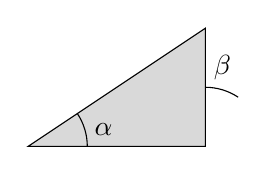
\begin{tikzpicture}[scale=1.5]
          \draw[fill=gray!30] (0,0) -- (1.5,0) -- (1.5,1) -- cycle;
          \draw (0.5,0) arc (0:33.69:0.5) node[midway,right] {$\alpha$};
          \draw (1.5,0.5) arc (90:56.31:0.5) node[midway,above] {$\beta$};
      \end{tikzpicture}
      \end{center}

      \textbf{Propriété :} Si $\alpha$ et $\beta$ sont deux angles complémentaires, alors $\alpha + \beta = 90^\circ$.

      \subsection{Angles Supplémentaires}

      \textbf{Définition :} Deux angles sont dits supplémentaires si leur somme est égale à $180^\circ$.

      \begin{center}
      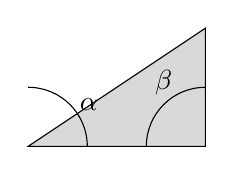
\begin{tikzpicture}[scale=1.5]
          \draw[fill=gray!30] (0,0) -- (1.5,0) -- (1.5,1) -- cycle;
          \draw (0.5,0) arc (0:90:0.5) node[midway,right] {$\alpha$};
          \draw (1.5,0.5) arc (90:180:0.5) node[midway,above] {$\beta$};
      \end{tikzpicture}
      \end{center}

      \textbf{Propriété :} Si $\alpha$ et $\beta$ sont deux angles supplémentaires, alors $\alpha + \beta = 180^\circ$.

      \subsection{Angles Adjacents}

      \textbf{Définition :} Deux angles sont dits adjacents si ils ont le même sommet, le même côté initial, mais des côtés finaux différents.

      \begin{center}
      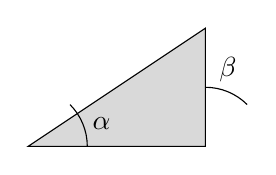
\begin{tikzpicture}[scale=1.5]
          \draw[fill=gray!30] (0,0) -- (1.5,0) -- (1.5,1) -- cycle;
          \draw (0.5,0) arc (0:45:0.5) node[midway,right] {$\alpha$};
          \draw (1.5,0.5) arc (90:45:0.5) node[midway,above] {$\beta$};
      \end{tikzpicture}
      \end{center}

      \textbf{Propriété :} Si $\alpha$ et $\beta$ sont deux angles adjacents, alors ils forment une paire linéaire et leur somme est égale.

    \fi











    \iffalse

        ooooooooooooooooooooooooo
                    O
                    O
                    O
                    O
                    O
                    O          OOOOOOOOOOO     OOOO
                    O          O               O   OO
                    O          OOOOO           O   OO
                    O          O               OOOO
                    O          O               0  0
                    O          OOOOOOOOOO      O   O

    \fi















    %\part{Terminale - Spé}



    %\setcounter{section}{0}






    \newpage


    \section{Raisonnement par Récurrence}

    \subsection{Concept générale}

    Le raisonnement par Récurrence est un raisonnement en trois phases : \textbf{Initialisation, Hérédité, Conclusion}
    qui vise à demontrer qu'une propriété $P_n$ est vrai $\forall n \in \mathbb{N}$.

    \subsection{Analogie des dominos}

    L'\textbf{Initialisation} consiste à prouver que le premier domino tombe.

    L'\textbf{Hérédité} consiste à prouver que si un domino donné tombe, alors le suivant tombera aussi.

    La \textbf{Conlcuion} consiste à conclure de ces deux faits que tout les dominos tombent.

    \subsection{Concept formel}


    \textbf{Initialisation} : On montre que la propriété est vraie pour la première valeur de \( n \), souvent notée \( n_0 \). Autrement dit, on prouve que $P_{n_0}$ est vérifiée.

    \textbf{Hérédité} : On suppose que la propriété est vraie pour un entier quelconque \( n \), et on montre qu'elle est alors vraie pour \( n + 1 \). En d'autres termes, on prouve que $P_n \Rightarrow P_{n+1}$.

    ~

    \textbf{Conclusion} : Si $P_{n_0}$ est verifiée et $\forall n \in \mathbb{N}, P_n \Rightarrow P_{n+1}$, alors $\forall n \in \mathbb{N}, P_n$ est vrai 


    \subsection{Remarques}

    \begin{itemize}
      \item La Récurrence peut être utile pour démontrer un \textbf{encadrement} et/ou une \textbf{variation} d'une suite DÉFINIE PAR RÉCURENCE.
      \item Faire attention aux moments où $n$ est général et quand il est un "entier naturel donné"

      
    \end{itemize}

    ~ \\ ~ \\

    Voir page suivante pour un exemple de raisonnement par Récurrence

    \newpage


    \subsection{Exemple de raisonnement par récurrence}

    On souhaite démontrer par récurrence la propriété :
    \[
    \forall n \in \mathbb{N}^*, ~~P_n : \sum_{k=1}^{n} k = \frac{n(n+1)}{2}
    \]

    \subsubsection{Étape 1 : Initialisation}

    Pour \( n = 1 \) :
    \[
    \frac{1 \times (1+1)}{2} = \frac{2}{2} = 1 = \sum_{k=1}^{1} k
    \]
    La propriété est donc vérifiée pour \( n = 1 \), $P_1$ est vérifiée.

    \subsubsection{Étape 2 : Hérédité}

    Supposons que la propriété est vraie pour un entier \( n \) quelconque, c'est-à-dire que :
    \[
      \sum_{k=1}^{n} k = \frac{n(n+1)}{2}
    \]
    On veut montrer qu'elle est alors vraie pour \( n + 1 \), c'est-à-dire que :
    \[
      \sum_{k=1}^{(n+1)} k = \frac{(n+1)(n+2)}{2}
    \]

    En ajoutant \( n + 1 \) des deux côtés de l'hypothèse de récurrence, on obtient :
    \[
      \sum_{k=1}^{n} k + (n + 1) = \frac{n(n+1)}{2} + (n + 1) = \frac{n(n+1) + 2(n+1)}{2}
    \]

    Factorisons par \( n+1 \):
    \[
      \sum_{k=1}^{(n+1)} k = \frac{(n+1)(n+2)}{2}
    \]

    On a donc montré que si la propriété est vraie pour un entier \( n \), elle l'est aussi pour \( n + 1 \).

    \subsubsection{Conclusion}

    On a prouvé que $P_1$ est vraie, et que $\forall n \in \mathbb{N}^*, P_n \Rightarrow P_{n+1}$, donc :
    \[
    \forall n \in \mathbb{N}^*, ~~P_n : \sum_{k=1}^{n} k = \frac{n(n+1)}{2}
    \]
    est verifiée.






    \newpage

    \section{Limites de fonctions}
    \label{sec:limFonction}

    \subsection{Limite d'une fonction à l'infini}
    \subsubsection{Limite infinie en \(\infty\)}
    On dit qu'une fonction \(f\) admet pour limite \(+\infty\) (resp. $-\infty$) en \(+\infty\) si \(f(x)\) a tout ses termes supérieures (resp. inferieurs) à tout réel A à partir d'un certain $x$.

    \subsubsection{Limite finie en \(\infty\)}
    La fonction \(f\) admet pour \textbf{unique} limite \(l\) en \(+\infty\) si \(f(x)\) se rapproche autant que l'on veut de $l$ à partir d'un certain $x$. On note alors : 
    \[
    \lim_{x \to +\infty} f(x) = l.
    \]
    La droite \(y = l\) est alors une asymptote horizontale.

    \subsection{Limite d'une fonction en un réel \(a\)}
      \subsubsection{Limite infinie en un point}
        Si \(f(x)\) devient aussi grand que l'on veut lorsque \(x\) s'approche de \(a\), alors on dit que \(f\) admet \(+\infty\) comme limite en \(a\). La droite \(x = a\) est une asymptote verticale à $f$.
      
      \subsubsection{Limite finie en un point}
      Si \(f(x)\) devient aussi proche que l'on veut d'un réel $l$ lorsque \(x\) s'approche de \(a\), alors on dit que \(f\) admet $l$ comme limite en \(a\). La droite \(y=l\) est une asymptote horizontale à $f$.

      \subsubsection{Limite à gauche et à droite}
        On distingue la limite à gauche ($x\to a, x<a$) et la limite à droite ($x\to a, x>a$), qui peuvent différer. Si elles sont égales, $l$ est l'unique limite en $a$

    \subsection{Opérations sur les limites}

    Soient $\displaystyle \lim_{x\to X} u_n ~\text{et} \lim_{x\to X} v_n ~ \text{dans} ~ \mathbb{R}\cup \{-\infty,+\infty\} $ de même que $X$. \\
    La limite en X de la somme, du produit, ou du quotient des suites \un et \vn est égal à la limite intuitive de la somme, du produit, ou du quotient de leurs limites en X, 
    à l'exception des \textbf{formes indéterminée} suivantes : 

    \[
    \begin{array}{c@{\hspace{2cm}}c@{\hspace{2cm}}c@{\hspace{2cm}}c}
    \displaystyle \bullet \ \frac{0}{0} & \displaystyle \bullet \ \frac{\infty}{\infty} & \displaystyle \bullet \ 0 \times \infty & \displaystyle \bullet \ +\infty - \infty
    \end{array}
    \]

    Lorsque la limite est déterminable, on a :

    \[
    \begin{array}{c@{\hspace{2cm}}c}
      \displaystyle \bullet \ \frac{k}{0^\pm} = \pm \infty & \displaystyle \bullet \ \frac{k}{\pm\infty} = 0^\pm \\[0.5cm]
      \displaystyle \bullet \ k \pm \infty = \pm \infty & \displaystyle \bullet \ k + 0^\pm = k^\pm
    \end{array}
    \] \vspace{0.3cm}

    \subsubsection{Théorèmes}

    Selon le \textbf{théorème de l'encadrement}, avec $(x,l)\in\mathbb{R}^2$ et $X\in\mathbb{R}\cup\{-\infty,+\infty\}$ : 
    \[
      \begin{cases} \exists \varepsilon \in \mathbb{R}, ~\forall x > \varepsilon,~ a(x)\le f(x) \le b(x) \\ \lim_{x\to X} a(x) = \lim_{x\to X} b(x) = l \end{cases} ~~ \Rightarrow ~~\lim_{x\to X} f(x) = l
    \]
    \newline

    Selon le similaire \textbf{théorème de comparaison}, avec $x\in\mathbb{R}$ et $X\in\mathbb{R}\cup\{-\infty,+\infty\}$ : 
    \[
      \begin{cases} \exists \varepsilon \in \mathbb{R}, ~\forall x > \varepsilon,~ a(x)\le f(x)\\ \lim_{x\to X} a(x) = +\infty \end{cases} ~~ \Rightarrow ~~\lim_{x\to X} f(x) = +\infty
    \]
    Et similairement, lorsque $f(x)\le a(x)$ et $\lim_{x\to X} a(x) = -\infty$, $\lim_{x\to X} f(x) = -\infty$ 
    \newline

    Enfin, selon le \textbf{théorème de croissance comparée}, pour tout entier naturel $n$ : 

    \[
    \lim_{x \to +\infty} \frac{e^x}{x^n} = +\infty ~~~~~~~ \text{et} ~~~~~~~ \lim_{x \to -\infty} x^n e^x = 0
    \]

    \[
      \lim_{x \to +\infty} \frac{\ln(x)}{x^n} = 0 ~~~~~~~~~ \text{et} ~~~~~~~ \lim_{x \to 0} x^n \ln(x) = 0
    \]


    Ces propriétés se bases sur l'inégalité suivante : 

    \[\forall x \in \R ~ , \quad e^x \ge x+1\]


    \subsection{Composition de fonctions}

      Soient $\mathcal{F}$ et $\mathcal{G}$ sous ensembles de $\R$ et soient $f$ et $g$ deux fonctions telles que $g : \mathcal{G} \to \mathcal{F}$ et $f : \mathcal{F} \to \mathbb{R}$. On définit sur $\mathcal{G}$ la fonction composée de $g$ suivie de $f$ par : 
      \[(f \circ g)(x) = f[g(x)]\]

      \subsubsection{Limite d'une composée}

      Soient $(a,b,c) \in \R \cup \{+\infty, -\infty\}$ , $f$ une fonction définie sur $I$, et $g$ une application quelconque (fonction, suite) à images dans $I$.

        \[\left\{\begin{array}{c}
          \displaystyle \lim_{x\to a} g(x) = b \\
          \displaystyle \lim_{x\to b} f(x) = c
        \end{array}\right.
        \quad \Rightarrow \quad
        \lim_{x\to a } (f \circ g)(x) =  c\]

    \subsection{Limites par taux d'accroissement (sup)}

    On peut obtenir des limites intéréssantes via la formule : 
    \[\lim_{x\to a} \frac{f(x) - f(a)}{x-a} \; = \; f'(a)\]

    Par exemple : 

    \[
    \begin{array}{c@{\hspace{2cm}}c@{\hspace{2cm}}c}
    \displaystyle \lim_{x\to0} \frac{e^x-1}{x} = 1 & \displaystyle \lim_{x\to0} \frac{\ln(x+1)}{x} = 1 & \displaystyle \lim_{x\to0} \frac{\sin(x)}{x} = 1
    \end{array}
    \]





    \newpage

    \iffalse\section{Géometrie dans l'espace}

    \subsection{Point}



    \subsection{Droite}



    \subsection{Plan}
    \fi
    \section{Géométrie dans l'espace}

    \subsection{Repère de l'espace}
    Un repère de l'espace est défini par un point d'origine $O$ et trois vecteurs non coplanaires $(\overrightarrow{i}, \overrightarrow{j}, \overrightarrow{k})$. Chaque point $M$ de l'espace est alors repéré par trois coordonnées $(x, y, z)$ telles que :
    \[
    \overrightarrow{OM} = x \overrightarrow{i} + y \overrightarrow{j} + z \overrightarrow{k}.
    \]

    \subsection{Vecteurs et droites dans l'espace}
    \subsubsection{Coordonnées d'un vecteur}
    Si $A(x_A, y_A, z_A)$ et $B(x_B, y_B, z_B)$ sont deux points de l'espace, alors le vecteur $\overrightarrow{AB}$ a pour coordonnées :
    \[
    \overrightarrow{AB} = \begin{pmatrix}
      x_B - x_A\\
      y_B - y_A\\
      z_B - z_A

    \end{pmatrix}
    \]

    \subsubsection{Equation paramétrique d'une droite}
    Une droite $D$ passant par un point $A(x_A, y_A, z_A)$ et dirigée par un vecteur directeur $\overrightarrow{u} (a, b, c)$ a pour \'{e}quations paramétriques :
    \[ (D) : 
    \begin{cases}
      x = x_A + \lambda a \\
      y = y_A + \lambda b \\
      z = z_A + \lambda c
    \end{cases}
    , \lambda \in \mathbb{R}
    \]

    \subsection{Plans dans l'espace}
    \subsubsection{Equation cartésienne d'un plan}
    Un plan $P$ passant par un point $A(x_A, y_A, z_A)$ et de vecteur normal $\overrightarrow{n} (a, b, c)$ a pour \'{e}quation cartésienne :
    \[
      \boxed{a(x - x_A) + b(y - y_A) + c(z - z_A) = 0.}
    \]

    \subsubsection{Intersection d'un plan et d'une droite}
    Une droite d'équation paramétrique intersecte un plan lorsque le système d'équations associé \`a leurs \'{e}quations possède une solution unique.


    \subsection{Colinéarité de deux vecteurs}

    Les deux vecteurs $\vec{AB}$ et $\vec{CD}$ sont colinéaires ssi : \[\boxed{\overrightarrow{AB} = k \cdot \overrightarrow{CD} ~~ , \quad k \in \R}\]
    On a alors que les droites $(AB)$ et $(CD)$ sont parrallèles, leurs points étant alignées si elles sont sécantes.




    \subsection{Produit scalaire et orthogonalité}
      \subsubsection{Produit scalaire de deux vecteurs}
        Soient $\overrightarrow{u}(x, y, z)$ et $\overrightarrow{v}(x',y',z')$ deux vecteurs, leur produit scalaire est donné par :
        
        \begin{empheq}[box=\fbox]{align*}
          \overrightarrow{u} \cdot \overrightarrow{v} &= x x' + y y' + z z' \\
                                                      &= ||\overrightarrow{u}|| \cdot ||\overrightarrow{v}|| \cdot \cos(\overrightarrow{u} ; \overrightarrow{v})
        \end{empheq}

      \subsubsection{Condition d'orthogonalité}
        Deux vecteurs sont orthogonaux si et seulement si leur produit scalaire est nul :
        \[
        \overrightarrow{u} \cdot \overrightarrow{v} = 0
        \]

      \subsubsection{Carré scalaire}

        \[\boxed{\vu^2 = ||\vu||^2}\]

      \subsubsection{Identités remarquables}

        \begin{empheq}[box=\fbox]{align*}
          (\vu \pm \vv)^2   &= \vu^2 + 2\uv + \vv^2 \\
          ||\vu \pm \vv||^2 &= ||\vu||^2 + 2\uv + ||\vv||^2
        \end{empheq}



    \subsection{Distances et angles dans l'espace}
    \subsubsection{Distance entre deux points}
    La distance entre deux points $A(x_A, y_A, z_A)$ et $B(x_B, y_B, z_B)$ est donnée par :
    \[
    AB = \sqrt{(x_B - x_A)^2 + (y_B - y_A)^2 + (z_B - z_A)^2}.
    \]

    \subsubsection{Angle entre deux vecteurs}
    L'angle $\theta$ entre deux vecteurs $\overrightarrow{u}$ et $\overrightarrow{v}$ est donné par la formule :
    \[
    \cos \theta = \frac{\overrightarrow{u} \cdot \overrightarrow{v}}{\|\overrightarrow{u}\| \|\overrightarrow{v}\|}.
    \]

    \subsection{Vecteur normal et projection orthogonale}
    \subsubsection{Vecteur normal d'un plan}
    Un vecteur normal au plan d'équation $ax + by + cz + d = 0$ est le vecteur $\overrightarrow{n} (a, b, c)$.

    \subsubsection{Projection orthogonale d'un point sur un plan}
    La projection orthogonale d'un point $M$ sur un plan est l'intersection de la droite passant par $M$ et orthogonale au plan avec ce dernier.


    \subsubsection{Milieu de $[AB]$}

      Soient $A$ et $B$ deux points distincts de l'espace et $I$ le milieu de $[AB]$.

      \[I \left(\frac{x_A+x_B}{2};\frac{y_A+y_B}{2};\frac{z_A+z_B}{2}\right)\]

    \subsection{Propriété}

      \begin{itemize}%[label=$\rightarrow$]
        \item \textbf{Deux plans sont perpendiculaires} lorsque l'un contient une droite orthogonale à l'autre
        \item \textbf{La distance d'un point $A$ à une droite $\mathcal{D}$} est $AH$ où H est le proj. horto. de $A$ sur $\mathcal{D}$. Soit $B$ un point de $\mathcal{D}$ et $\vu$ un vecteur directeur de cette droite : 
                \[
                    \boxed{AH = \left\lVert \overrightarrow{AB} - 
                    \frac{\overrightarrow{AB}\cdot \vu}{\lVert \vu \rVert^2}\,\vu \right\rVert}
                \]
        
        \item \textbf{La distance d'un point $A$ à un plan $\mathcal{P}$} est $AH$ où H est le proj. horto. de $A$ sur $\mathcal{P}$. Soit $B$ un point de $\mathcal{P}$ et $\overrightarrow{n}$ un vecteur normal à ce plan : 
                \[
                    \boxed{AH = \frac{|\overrightarrow{AB}\cdot \overrightarrow{n}|}{\lVert \overrightarrow{n} \rVert}}\]
      \end{itemize}












    ~~ \newline ~~ \newline

    \section{Compléments de géometrie : angles orientés}

      Plaçons nous dans un repère orthonormé direct $(O ; \overrightarrow{OI} ; \overrightarrow{OJ})$. Soit $x$ un réel et $M$ son image sur le cercle trigonométrique.

      \begin{itemize}[label=$\rightarrow$]
        \item $x$ est une mesure de l'angle orienté $(\overrightarrow{OI} ; \overrightarrow{OM})$
        \item on défini $\nu$ la \textbf{mesure principale} de l'angle orienté $(\overrightarrow{OI} ; \overrightarrow{OM})$ par : \[\nu = x [2\pi] - \pi\] de sorte à ce que $\nu$ appartiennes à l'intervalle $]-\pi; \pi]$
      \end{itemize}

      \subsection*{Radians}

      Soient $x$ un angle en radians, et $\alpha$ son equivalent en degrés. On a que : 

      \[\frac{x}{\pi} = \frac{\alpha}{180}\]

    \section{Compléments de géometrie : cerlces du plan}

      Un cercle du plan est caractérisé par une équation du type :
      \[(x-x_0)^2 + (y-y_0)^2 = r^2\]

      D'où la forme $x^2+y^2 = 1 $ pour le cercle trigo.

      La longueure $AB$ d'un arc entre $A$ et $B$ d'un cercle de rayon $r$, l'angle $\theta$ séparant $A$ et $B$ : 

      \[\wideparen{AB} = r\theta \quad , \quad \theta = (\overrightarrow{OA},\overrightarrow{OB})\]










    \newpage









    \section{Primitives}

      \subsection{Primitives de fonctions usuelles}

      \begin{center}
        \renewcommand{\arraystretch}{2.25}
        \begin{tabular}{|c|c|c|}
          \hline
          \textbf{Fonction $f$ sur $I$} 
          & \textbf{$F_0$ de $f$ sur $I$} 
          & \textbf{Ensemble $I$} \\
          \hline
          $k$ (constante réelle) & $kx$ & $\mathbb{R}$ \\
          \hline
          $x$ & $\frac{1}{2} x^2$ & $\mathbb{R}$ \\
          \hline
          $x^n$ ($n \in \mathbb{Z}\backslash\{0;-1\}$) 
          & $\frac{1}{n+1} x^{n+1}$ 
          & $\mathbb{R}$ si $n > 0$,\newline $\mathbb{R}^*$ si $n < -1$ \\
          \hline
          $\dfrac{1}{x^2}$ & $-\dfrac{1}{x}$ & $\mathbb{R}^*$ \\
          \hline
          $\dfrac{1}{\sqrt{x}}$ & $2 \sqrt{x}$ & $\mathbb{R}^*_+$ \\
          \hline
          $\dfrac{1}{x}$ & $\ln(x)$ & $\mathbb{R}^*_+$ \\
          \hline
          $e^x$ & $e^x$ & $\mathbb{R}$ \\
          \hline
        \end{tabular}
      \end{center}

      L'ensemble des primitives de $f$ sur $I$ est l'ensemble des fonctions $F$ définies sur $I$ par : 
      \[\boxed{F : x \to F_0(x) + \mathcal{C}} ~ , \quad \mathcal{C} \in \R\]

      \iffalse\subsection{Primitives et opérations}

      Soient $f$ et $g$ deux fonctions ayant respectivement pour primitives $F$ et $G$ sur un intervalle $I$, et soit $k$ un réel :
      \begin{itemize}
        \item Une primitive de $f + g$ sur $I$ est $F + G$.
        \item Une primitive de $k f$ sur $I$ est $k F$.
      \end{itemize}\fi

      \subsection{Primitives et composition}

        Soit $u$ et $v$ deux fonction dérivable sur $I$ et $n \in \mathbb{Z} \setminus \{[0, -1]\}$ :

        \begin{center}
          \renewcommand{\arraystretch}{2.25}
          \begin{tabular}{|c|c|c|}
            \hline
            \textbf{Forme} & \textbf{Une primitive est} & \textbf{Conditions} \\
            \hline
            $u' + v'$ & $u + v$ & - \\
            \hline
            $ku'$ & $ku$ & $k\in\mathbb{R}$ \\
            \hline
            $u' \cdot u^n$ 
            & $\dfrac{1}{n+1} u^{n+1}$ 
            & $u \ne 0$ sur $I$\\% et $n > 0$ ou $n < -1$\\
            \hline
            $\dfrac{u'}{u^2}$ & $- \dfrac{1}{u}$ & $u \ne 0$ sur $I$ \\
            \hline
            $\dfrac{u'}{u}$ & $\ln(u)$ & $u > 0$ sur $I$ \\
            \hline
            $\dfrac{u'}{\sqrt{u}}$ & $2 \sqrt{u}$ & $u > 0$ sur $I$ \\
            \hline
            $u' \cdot e^u$ & $e^u$ & $u$ dérivable sur $I$ \\
            \hline
          \end{tabular}
        \end{center}

      \subsection{Remarques}

        \begin{itemize}
          \item penser à jongler entre $\frac{1}{u^n}$ et $u^{-n}$
          \item $\cdots$ $F+G$ est primitive de $f+g$ et $kF$ est primitive de $kf$
        \end{itemize}




    \newpage

    \section{Equations différentielles}

      \subsection{Définition}

        Une équation différentielle est une équation dont l'inconnue $y$ est une fonction.
        Une équation différentielle mettant en jeu une fonction et ses $n$ premièrs dérivées est dite \textbf{d'ordre $n$}.

      \subsection{Forme $y' = f$, primitive}

        Soit $f$ fonction continue sur I. Cette équation a pour solution l'ensemble des primitives de la fonction $f$ sur I telles que, pour tout $x$ de I, $F'(x) = f(x)$. On a donc, avec $F_0$ une primitive de $f$ : 

        \[\boxed{y = F_0(x) \pc}\]

        solution de (E). 
        \begin{itemize}
          \item On note que \textbf{toute fonction continue sur I admet des primitives sur I}.
          \item \textbf{Condition initale} : soient $x_0 \in I$, $y_0 \in \mathbb{R}$, $\boxed{\exists ! ~F : I \to \mathbb{R} ~, ~~F(x_0) = y_0}$
        \end{itemize}

      \iffalse\subsection{Forme $y' = a y$}

        La solution générale est donnée par :
        \[\boxed{y(x) = C e^{a x}}\]
        où $C \in \mathbb{R}$ est une constante d'intégration.
        \fi

      \subsection{Equadiff de 1er ordre à coeff constant, forme :  $y' = a y + b$}

        La solution générale est donnée par :

          \[
          \boxed{y(x) = C e^{a x} - \dfrac{b}{a}} \quad C \in \mathbb{R} , a \ne 0
          \]

        \iffalse\paragraph{Cas particulier $a = 0$ :}
        \[
        y' = b \Rightarrow y = bx + C
        \]\fi

        \subsection{Equadiff de 1er ordre à coeff variable, forme :  $y' = a y + f$}

        La solution générale est donnée par :

          \[
          \boxed{y(x) = C e^{a x} + f_0(x)} \quad C \in \mathbb{R} , f : \mathbb{R} \to \mathbb{R}
          \]



      \subsection{Propriétés des solutions}

        \begin{itemize}
          \item L'ensemble des solutions d'une équation différentielle linéaire de premier ordre $y' = a y + b$ forme une \textbf{famille affine de fonctions}.
          \item La solution est \textbf{unique} si une condition initiale est imposée.
        \end{itemize}





    \newpage

    \section{Intégration}

    \subsection{Définition}

    Soit \( f \) une fonction continue sur \( I = [a, b] \) et \( \mathcal{C} \) sa courbe représentative. L'aire du domaine \( \mathcal{D} \) entre \( \mathcal{C} \) et l'axe des abscisses, et entre les verticales en \( a \) et en \( b \) est appelée intégrale de \( a \) à \( b \) de \( f \) et est notée :

      \[
        \int_{a}^{b} f(x) \, dx
      \]
    \subsection{Théoreme d'éxistence d'une primitive}

      Soient $f$ une fonction continue sur un intervalle $I$, alors la fonction $\phi$ def sur $I$ par $\displaystyle\phi(x) = \int_{a}^{b}f(x)dx$ est l'unique primitive de $f$ sur $\left[a ~; b\right]$ s'annulant en $x=a$.

    \subsection{Calcul d'intégrale}

      Soit $f$ une fonction \textbf{continue} sur $\left[a ~; b\right]$, et $F$ une primitive de $f$ sur $\left[a ~; b\right]$ : 

      \[\boxed{\int_{a}^{b}f(x)dx = \Bigl[ F(x) \Bigr]^b_a = F(b) - F(a)}\]


    \subsection{Propriétés des intégrales}

      Soient \( a \) et \( b \) deux réels tels que \( a < b \), et soient \( f \) et \( g \) deux fonctions continues sur l’intervalle \( [a ; b] \). On note \( F \) une primitive de \( f \) sur cet intervalle.

      \paragraph{Linéarité}
      \[
      \int_a^b k \cdot f(x) \, dx = k \cdot \int_a^b f(x)\, dx
      \]
      \[
      \int_a^b \left( f(x) + g(x) \right) dx = \int_a^b f(x)\, dx + \int_a^b g(x)\, dx
      \]

      \iffalse\paragraph{Relation de Chasles}
      Pour tout \( c \in [a ; b] \) :
      \[
      \int_a^b f(x)\, dx = \int_a^c f(x)\, dx + \int_c^b f(x)\, dx
      \]
 
      \paragraph{Positivité}
      \begin{itemize}
        \item Si \( f(x) \geq 0 \) sur \( [a ; b] \), alors \( \int_a^b f(x)\, dx \geq 0 \)
        \item Si \( f(x) < 0 \) sur \( [a ; b] \), alors \( \int_a^b f(x)\, dx < 0 \)
      \end{itemize}\fi

      \paragraph{Intégration des inégalités}
      \[
      \text{Si, pour tout } x \in [a ; b],~ f(x) \leq g(x), \text{ alors } \int_a^b f(x)\, dx \leq \int_a^b g(x)\, dx
      \]
      \textit{Attention : la réciproque est fausse.}

      \paragraph{Intégration par parties}
        \[
        \boxed{\int_a^b u(x)\,v'(x)\, dx = \left[ u(x)\,v(x) \right]_a^b - \int_a^b u'(x)\,v(x)\, dx}
        \]

      \paragraph{Positivité de l'intégral}
        \begin{itemize}
          \item $f$ positive sur $[a ; b] ~~~ \Rightarrow ~~ \int_a^b f(x)\, dx \geq 0$
          \item $f$ négative sur $[a ; b] ~~~ \Rightarrow ~~ \int_a^b f(x)\, dx \leq 0$
        \end{itemize}

      \newpage

      \subsection{Applications du calcul intégral}

      \paragraph{1. Valeur moyenne d'une fonction}
      Soit \( f \) une fonction continue sur un intervalle \( [a ; b] \). La valeur moyenne de \( f \) sur cet intervalle est :
      \[
      m = \frac{1}{b - a} \int_a^b f(x)\, dx
      \]

      Le théorème des valeures intermetières permet d'assurer l'existence d'un réel $c \in \left[a:b\right]$ tel que : 
      \[f(c) = m\]

      \textit{Remarque} : dans le cas où \( f \) est continue et positive sur \( [a ; b] \), ce nombre \( m \) représente la hauteur du rectangle de base \( [a ; b] \) et de même aire que le domaine délimité par la courbe de \( f \), l’axe des abscisses et les droites \( x = a \) et \( x = b \).

      \paragraph{2. Aire entre deux courbes}
      Soient \( f \) et \( g \) deux fonctions continues et positives sur un intervalle \( [a ; b] \), telles que :
      \[
      \forall x \in [a ; b],\quad f(x) \leq g(x)
      \]
      Alors l’aire, exprimée en unités d’aire, de la surface comprise entre les courbes de \( f \) et \( g \), et les droites \( x = a \) et \( x = b \), est :
      \[
      \mathcal{A} = \int_a^b \left( g(x) - f(x) \right) dx
      \]

      De façon plus générale, pour toutes fonctions $f$ et $g$ continues sur $\left[a;b\right]$ : 
      \[
        \mathcal{A} = \int_a^b | g(x) - f(x) | dx
      \]










    \newpage



\section{Dénombrement}

\subsection{Les Principes de Base}

Soient $A$ et $B$ deux ensembles, et $|A| = Card(A)$

\iffalse\subsubsection{Principe Additif}
Si deux ensembles \( A \) et \( B \) sont disjoints, alors le nombre d'éléments dans \( A \cup B \) est égal à la somme du nombre d'éléments dans \( A \) et du nombre d'éléments dans \( B \).

\[ |A \cup B| = |A| + |B| \]\fi

\subsubsection{Principe Multiplicatif}
\label{princMul}
Si un événement peut se produire de \( n \) manières différentes et qu'un second événement peut se produire de \( m \) manières différentes, alors les deux événements peuvent se produire de \( n \times m \) manières différentes.

\[ |A \times B| = |A| \times |B| \]

\subsubsection{Produit Cartésien}

        \begin{itemize}
          \item Soient $\mathcal{E}_k$ k ensembles non vides. $\mathcal{E}_1 \times \mathcal{E}_2 \times \cdots \times \mathcal{E}_k$ est appelé produit cartésien des $\bigEps_k$, et représente l'ensemble des k-uplets formés par les éléments des $\bigEps_k$.
          \item Soient $\bigEps$ un ensemble et $k\in\mathbb{N}$. Selon le \nameref{princMul} : \[|\bigEps^k| = |\bigEps|^k\]
        \end{itemize}

\subsubsection{Parties de $\bigEps$}

        Soit $\mathfrak{B}(\bigEps)$ l'ensemble des parties de $\bigEps$, ensemble de $k$ éléments : \(|\mathfrak{B}(\bigEps)| = 2^k\)

        

\subsection{Permutations}

  \subsubsection{Définition}
    Une permutation d'un ensemble \( E \) de \( n \) éléments est un arrangement de tous les éléments de \( E \). On en dénombre :

    \[ P_n = n! \]

\subsection{Arrangements}

\subsubsection{Définition}
Un arrangement de \( k \) éléments d'un ensemble \( E \) de \( n \) éléments est une liste ordonnée de \( k \) éléments distincts de \( E \). On en dénombre :

\[ A_n^k = \frac{n!}{(n-k)!} \]

\subsection{Combinaisons}

\subsubsection{Définition}
Une combinaison de \( k \) éléments d'un ensemble \( E \) de \( n \) éléments est une sélection non ordonnée de \( k \) éléments distincts de \( E \). On en dénombre : 

\[ C_n^k = \binom{n}{k} = \frac{n!}{k!(n-k)!} \]

Il s'agit du nombre de chemin dans un arbre binaire $A$/$B$ à $n$ niveaux contenant exactement $k$ noeuds $A$.

\iffalse\subsubsection{Exemple}
Combien de mains de 5 cartes peut-on tirer d'un jeu de 32 cartes ?

\[ C_{32}^5 = \binom{32}{5} = \frac{32!}{5!(32-5)!} = 201376 \]
\fi

\iffalse\subsubsection{Exemple}
Développer \( (x + y)^3 \) :

\[ (x + y)^3 = \binom{3}{0} x^3 y^0 + \binom{3}{1} x^2 y^1 + \binom{3}{2} x^1 y^2 + \binom{3}{3} x^0 y^3 \]
\[ = x^3 + 3x^2y + 3xy^2 + y^3 \]\fi

\subsection{MindMap}

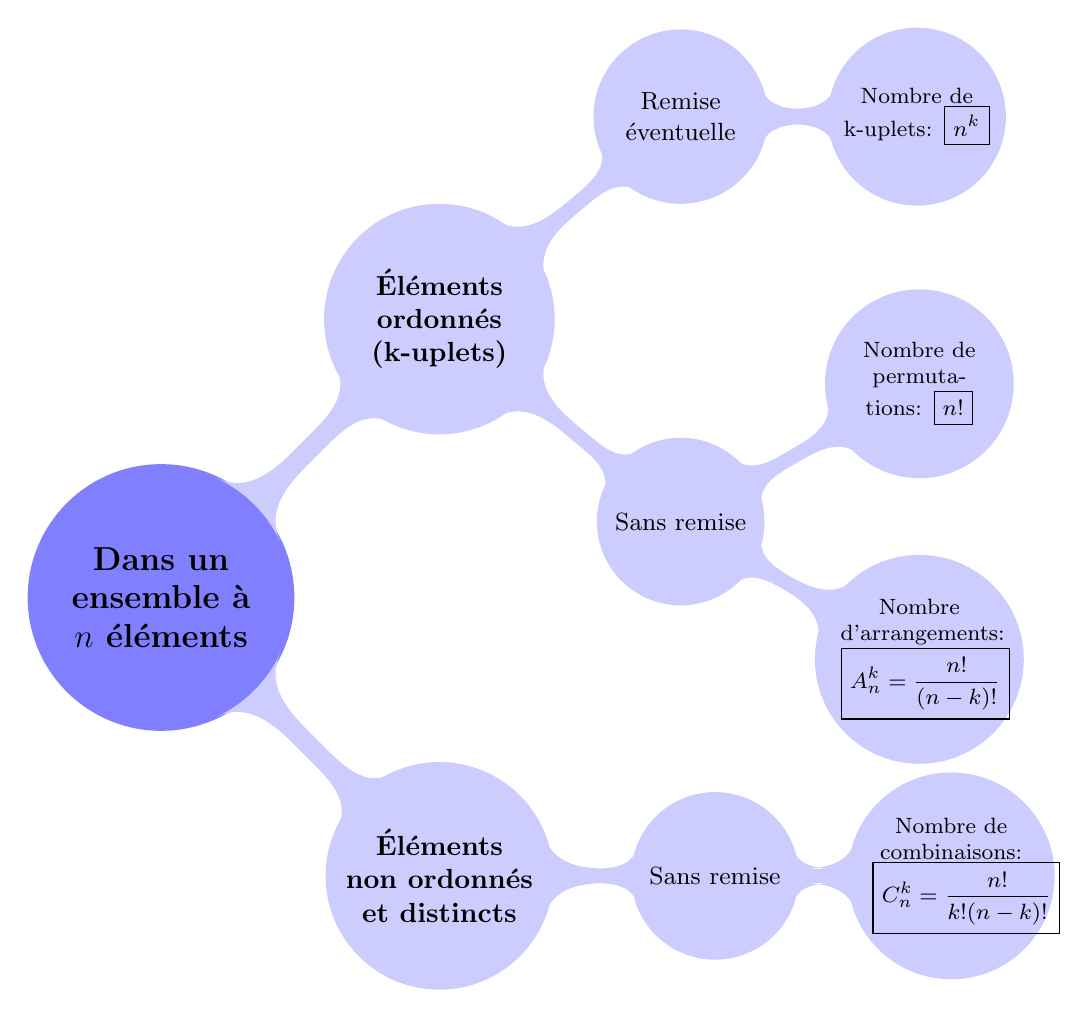
\begin{tikzpicture}[
  mindmap,
  concept color=blue!20,
  every node/.style={concept},
  root concept/.append style={
    concept color=blue!50, font=\large\bfseries, minimum size=3cm, text width=3cm},
  level 1 concept/.append style={font=\bfseries, sibling angle=120, minimum size=2.5cm, text width=2.5cm},
  level 2 concept/.append style={font=\small, sibling angle=60, minimum size=2cm, text width=2cm},
  level 3 concept/.append style={font=\footnotesize, sibling angle=60, minimum size=1.5cm, text width=2cm}
]

\node [root concept] {Dans un ensemble à $n$ éléments}
  child [grow=45, level distance=5cm] { node {Éléments ordonnés (k-uplets)}
    child [grow=40, level distance=4cm] { node {Remise éventuelle}
        child [grow=0, level distance=3cm] { node {Nombre de k-uplets: $\boxed{n^k}$} }
    }
    child [grow=-40, level distance=4cm] { node {Sans remise}
        child [grow=30, level distance=3.5cm] { node {Nombre de permutations: $\boxed{n!}$} }
        child [grow=-30, level distance=3.5cm] { node {Nombre d'arrangements: $\boxed{A_n^k = \frac{n!}{(n-k)!}}$} }
    }
  }
  child [grow=-45, level distance=5cm] { node {Éléments non ordonnés et distincts}
    child [grow=0, level distance=3.5cm] { node {Sans remise}
      child [grow=0, level distance=3cm] {node {Nombre de combinaisons: $\boxed{C_n^k = \frac{n!}{k!(n-k)!}}$}}
    }
  };

\end{tikzpicture}

\newpage


\part{CPGE - PTSI}

\section*{NB} 
Cette partie est complémentaire de la première, ce qui implique qu'une partie des cours dispensés en maths niveaux prépa sont en réalité des compléments à des notions étudiées au lycée, et les chapitres concernés ont donc été mis à jour, plutot que d'encombrer cette partie. \\
Il est donc nécéssaire de maitriser les notions de la partie précédente, qui sont soit nécéssaire à la compréhension et au maniement des outils plus avancés, soit sont déjà considérées comme faisant partie prennante du programme de classe prépa.

\newpage

\setcounter{section}{0}

\section{Révisions sur les nombres réels}

XX Ficher limites par taux d'accroissement XX

Bien connaitre les \nameref{IDR} 3eme deg et $(a+b+c)^2$ \\~\\

\paragraph{Def scalaire} Constante de $\R$ ou $\mathbb{C}$.


\newpage


\section{Systèmes linéaires sur $\R^2$ et $\R^3$}

  \subsection{Définitions}

    On appelle \textbf{système linéaire de $n$ équation à $p$ inconnues} tout système d'équation de la forme : 

    \[(S) = \left\{\begin{array}{c}
      a_1x_1+a_2x_2+\cdots+a_p+x_p = a_S \\
      b_1x_1+b_2x_2+\cdots+b_p+x_p = b_S \\
      \cdots \\
      \omega_1x_1+\omega_2x_2+\cdots+\omega_p+x_p = \omega_S
    \end{array}\right.\]

    où : 
    \begin{itemize}
      \item $x_i$ les \textbf{inconnues}
      \item $a_i, b_i, \cdots, \omega_i$ des \textbf{coefficients} réels
      \item $a_S, b_S, \cdots, \omega_S$ les \textbf{seconds membres} des équations
    \end{itemize}

    \subsubsection*{Divers définitions}

      \begin{itemize}
        \item \textbf{Résoudre le système $(S)$} est trouver l'ensemble des $p$-uplets dits \textbf{solutions dS}
        \item Deux systèmes sont dit \textbf{équivalents} si ils ont le même $\mathcal{S}$. Alors : $(S) \Leftrightarrow (S')$
        \item On appelle \textbf{opération élémentaire} toute opération \underline{réversible}\footnote{\textbf{Dem :} on trouve trivialement l'opération réciproque de chacune} consistant à :
        \begin{itemize}[label=$\rightarrow$]
          \item \begin{tabular*}{\linewidth}{@{\extracolsep{\fill}} l r}
                  \textbf{échanger} deux lignes & $L_i \leftrightarrow L_j$
                \end{tabular*}
          \item \begin{tabular*}{\linewidth}{@{\extracolsep{\fill}} l r}
                  \textbf{multiplier} une ligne \textbf{par un scalaire}$^*$ & $L_i \leftarrow \alpha L_i$
                \end{tabular*}
          \item \begin{tabular*}{\linewidth}{@{\extracolsep{\fill}} l r}
                  \textbf{ajouter} un multiple d'une ligne à une autre & $L_i \leftarrow L_i + \alpha L_j$
                \end{tabular*}
          \item combinaison de ces deux dernières
        \end{itemize}
      \end{itemize}

  
  \air
    

  \subsection{Méthode du pivot de Gauss}
   

    Par une suite finie d'opérations élémentaires sur les lignes, on transforme le système linéaire $\Sys$ en un système linéaire équivalent $(S')$ \underline{échelonné} : 

    \iffalse\begin{center}
      \includegraphics[width=0.6\textwidth]{images/pivot.png}
    \end{center}\fi

    \[
      \begin{cases}
        ax ~ + by ~= c \\
        a'x + b'y = c'
      \end{cases}
      \;\; \xLongrightarrow{\,L_2 \leftarrow L_2 + \alpha L_1\,} \;\;
      \begin{cases}
        ax + by = c \\
        ~~~~~~~ dy = e
      \end{cases}
    \]\vspace{0.5em}


    On appelle \textbf{pivot} le premier coefficient non nul de chaque équation du système. On obtient les solutions de $\Sys$ par remontés successives.



    \newpage

    
  
  \subsection{Interprétation géométrique}

    \subsubsection{Droite du plan}

      On se place dans un plan muni d'un repère orthonormé $(O,\vec{i},\vec{j})$.\\
      $\forall (a,b)\in(\R^2)^*$ l'équation $\boxed{ax+by=c}$ est celle d'une droite de vec. dir. $\boxed{u=(-b~,~a)}$ et de vec. normal $\boxed{u=(a~,~b)}$
      
      Réciproquement toute droite du plan admet une equation de ce type.

    \subsubsection{Plan de l'espace}

      Avec $a,b,c,d\in\R$ et $(a,b,c)\ne(0,0,0)$ ; $\boxed{ax+by+cz+d}$ est l'équation cartésienne d'un plan de l'espace $\R^3$, de vec. normal $n=(a,b,c)$.
      
      Réciproquement tout plan de l'espace $\R^3$ admet une telle equation.

    \subsubsection{Résolution d'un système (2,2)}

      Soit : 
      \[(S) \; \begin{cases}
        ax+~by~=c ~~~~~ (\Delta_1)\\
        a'x+b'y=c' ~~~~~ (\Delta_2)
      \end{cases}\]

      Résoudre $\Sys$ (2,2) revient à la recherche des intersections des deux droites du plan. Il y a donc trois cas possibles :
      \begin{itemize}
        \item droites // $\iff$ $\mathcal{S} = \emptyset$ ~~~~~~~~~~~~~~~~~~~~~~~~~$\iff$ $(a,b) = k(a',b')$
        \item droites /~~ $\iff$ $\mathcal{S} = \left\{(x,y) | ax+by=c\right\}$ $\iff$ $\Delta_1 = k\Delta_2$
        \item droites X ~$\iff$ $\mathcal{S} = ~!(x,y)$%~~~~~~~~~~~~~~~~~~ $\iff$ $\Delta_1 = k\Delta_2$
      \end{itemize}

    \subsubsection{Note : systèmes (3,2)}

      Les système (n,p) où n>p peuvent être \textbf{hyperstatiques}, i.e. posséder \underline{trop} de contraintes et ainsi n'avoir aucune solution. Dans le cas d'un système (3,2), ce cas correspond à l'éventualité où les trois droites ne concourent pas en un unique point et ne sont pas toutes trois confondus.


    \subsubsection{Résolution d'un système (2,3)}

      Soit : 
      \[(S) \; \begin{cases}
        ax+~by~+cz~=d ~~~~~ (\mathcal{P}_1)\\
        a'x+b'y+c'z=d' ~~~~~ (\mathcal{P}_2)
      \end{cases}\]

      Résoudre $\Sys$ (2,3) revient à la recherche des intersections des deux plans de l'espace. Il y a donc trois cas possibles :
      \begin{itemize}
        \item plans // $\iff$ $\mathcal{S} = \emptyset$ ~~~~~~~~~~~~~~~~~~~~~~~~~~~~~~~~~~$\iff$ $(a,b,c) = k(a',b',c')$
        \item plans /~~ $\iff$ $\mathcal{S} = \left\{(x,y,z) | ax+by+cz=d\right\}$ $\iff$ $\mathcal{P}_1 = k\mathcal{P}_2$
        \item plans X ~$\iff$ $\mathcal{S} = ~!(x,y,z)$
      \end{itemize}

    \subsubsection{Méthode générale}

      L'acception géométrique peut permettre de rapidement ``\textbf{discuter}'' la nature des solutions, nottament via les vec. normaux, et directeurs


  \section{Ensemble des nombres réels}

    \subsection{Ensemble des nombres réels}

      On se permettra d'admettre la connaissance des parties remarquable de $\R$. \\
      On notera cependant les curiosités suivantes : 

      \subsubsection{Démonstration de l'irrationnalité de $\sqrt{2}$}

      \begin{tcolorbox}[colback=white, colframe=black, boxrule=0.8pt, width=1\textwidth]

        Supposons, par l'absurde, que \(\sqrt{2}\) soit rationnel. Alors il existe des entiers relatifs \(p\) et \(q\) (avec \(q\neq0\)) tels que
        \[
        \sqrt{2}=\frac{p}{q},
        \]
        et on peut choisir cette fraction sous forme irréductible, c'est-à-dire \(\pgcd(p,q)=1\).

        En élevant au carré on obtient
        \[
        2=\frac{p^2}{q^2}\quad\Longrightarrow\quad p^2=2q^2.
        \]
        Donc \(p^2\) est pair, ce qui implique que \(p\) est pair. On peut donc écrire \(p=2k\) pour un certain entier \(k\). En remplaçant dans l'égalité précédente :
        \[
        (2k)^2=2q^2 \quad\Longrightarrow\quad 4k^2=2q^2 \quad\Longrightarrow\quad q^2=2k^2.
        \]
        Ainsi \(q^2\) est pair, donc \(q\) est pair.

        Nous avons donc montré que \(p\) et \(q\) sont tous deux pairs, ce qui contredit l'hypothèse que la fraction \(\dfrac{p}{q}\) soit irréductible (\(\pgcd(p,q)=1\)). Cette contradiction montre que l'hypothèse initiale était fausse.

        Par conséquent : \(\boxed{\sqrt{2}\ \text{est irrationnel}.}\)

      \end{tcolorbox}

    \subsection{Inégalités dans $\R$}

      \subsubsection{Définitions}

        \begin{itemize}[label=$\rightarrow$]
          \item On dit que $x\le y $ (resp. $\ge$) si $x-y\in\R_-$ (resp. $\R_+$) ; \\ $\R^*_{\cdots}$ pour les inégalités stricts
          \item Géométriquement, si M:(x) et N:(y) ;  $x\le y $ (resp. $\ge$) si $\overrightarrow{MN}$ et $\vec{i}$ de même sens (resp. de sens contraire)
        \end{itemize}

        \subsubsection{Relation d'ordre}

          On appelle \textbf{relation d'ordre} une relation qui est \underline{réflexive}, \underline{antisymétrique}, et \underline{transitive}.
          
          Exemple : la relation \(\le\) sur \(\mathbb{R}\).
          
          \begin{itemize}
            \item \textbf{Réflexive : } \(\forall x \in \mathbb{R}, \; x \leq x\).
            \item \textbf{Antisymétrique : } \(\forall x,y \in \mathbb{R}, \; (x \leq y \;\wedge\; y \leq x) \;\Rightarrow\; x=y\).
            \item \textbf{Transitive : } \(\forall x,y,z \in \mathbb{R}, \; (x \leq y \;\wedge\; y \leq z) \;\Rightarrow\; x \leq z\).
          \end{itemize}

          $\le$ est une relation d'ordre \textbf{totale}, car $\forall x,y\in \R \, , \; x\le y \lor y\le x$


  \newpage

  \section{Arithmétique}

    \subsection{Divisibilité et division}

      \subsubsection{Divisibilité sur $\N$ et $\Z$}

          Soient $n,p\in\Z$. On dit que \textbf{n divise p} ou \textbf{n est multiple de p}, si $n = kp \, , \, k\in\Z$. Ainsi : 

          \setlength{\fboxsep}{5pt} % default 3pt
          \[
          \boxed{\left(a \mid p\right) \iff \left(\exists k \in \mathbb{Z}, \; n = kp\right)}
          \]

          \paragraph{Rq} La divisibilité sur $\Z$ est refléxive et transitive, mais pas antisymétrique, ce n'est donc pas une relation d'ordre sur $\Z$. C'est cependant le cas sur $\N$ où elle est partielle ($3\not|~7$ et $7\not|~3$)



      \subsubsection{Division euclidienne sur $\N$}

          \paragraph{Théorème} Soient $n,p\in\N^*$ 

            \[
              \boxed{\exists! (q,r) \in \mathbb{N}^2, \quad n = qp + r ~~, \quad 0\le r<p}
            \]

          \paragraph{Démonstration}~\\

          \setlength{\fboxsep}{4pt} % default 3pt

          \begin{tcolorbox}[colback=white, colframe=black, boxrule=0.8pt, width=1\textwidth]

            \begin{itemize}
              \item \textbf{existence : } Avec $n\in\N^*$, nottons $E=\left\{a\in\N \,|\, ap < n\right\}$. $E$ est une partie non vide (contient 0) et majorée (par $n$) de $\N$. Donc $E$ admet un maximum. 

                    Notons $\boxed{q = \text{max}(E)}$ ce maximum et $\boxed{r = n-pq}$

                    Alors : 
                    \[\begin{cases}
                      q\in\N \, , \, r\in\N \\
                      n = pq + r
                    \end{cases} 
                    ~\text{et}~~~ 
                    \begin{cases}
                      q\in E ~~~~~~ \Rightarrow ~~ pq \le n ~~~~~~~~\text{et}~~ r = n-pq \ge 0\\
                      q+1\not\in E ~ \Rightarrow ~~ p(q+1) > n ~\text{et}~~ r = n-p(q+1) < p 
                    \end{cases}\]

                    On a donc bien $\exists q,r \in \mathbb{N}, \quad n = qp + r ~~, \quad 0\le r<p$
                \item \textbf{unicité : } Soient $(q_1, r_1)$ et $(q_2, r_2)$ deux couples de $\mathcal{S}$

                    \[\begin{cases}
                      n = pq_1 + r_1 \\
                      0\le r_1 < p 
                    \end{cases}
                    ~\text{et}~~~~ 
                    \begin{cases}
                      n = pq_2 + r_2 \\
                      0\le r_2 < p \iff -p < -r_2 \le 0
                    \end{cases}\]

                    On en déduit : \(\begin{cases}
                      r_2-r_1 = p (q_1 - q_2)\\
                      -p<r_2-r_1<p
                    \end{cases}\) \\
                    Or le seul entier multiple de $p$ et strictement entre $-p$ et $p$ est 0\footnote{Selon le système précédent, $\Delta r = p \Delta q$ donc $\Delta r$ multiple de $p$ et donc $|r_2-r_1|\ge p$ ; \newline mais on a également : ~~~~~~~~~~~ $-p < r_2-r_1 < p$ ~~~~~~~~~~~~~~~~~~~~~~~~ donc $|r_2-r_1| < p$},
                    donc $r_2-r_1 = 0$ d'où $r_1=r_2$ puis $q_1=q_2$.

                    D'où l'unicité du quotient et du reste de la division euclidienne de $n$ par $p$.
            \end{itemize}
          
          \end{tcolorbox}

      \paragraph{Rq} On peut élargir la définition à $\Z$.

      \paragraph{Proposition} \textbf{La reste vérifie : } $\boxed{r=0 \iff p|n}$

      \subsubsection{Nombres premiers}

        \begin{itemize}
          \item \textbf{Définition}
            \begin{itemize}[label=$\rightarrow$]
              \item Un entier naturel est un \underline{nombre premier} s'il n'est divisible dans $\N$ que par 1 et lui-même. 
              \item 1 n'est pas premier.
            \end{itemize}
          \item \textbf{Proposition}
            \begin{itemize}[label=$\rightarrow$]
              \item Tout entier naturel distinct de 0 et 1 \underline{admet au moins un diviseur premier}.
              \item Si $n$ n'est pas premier, il admet au moins un diviseur premier $p$ tel que : \[p^2\le n\].
            \end{itemize}

          \item \textbf{Démonstration} : HP de Colles, à ficher un jour
          \item \textbf{Crible d'Eratosthène}
            \begin{center}
              \includegraphics[width=0.6\textwidth]{images/eratosthene.png}
            \end{center}
            \begin{itemize}[label=$\rightarrow$]
              \item On entoure le + petit disponible (premier) et on barre tout ses multiples (\underline{composés}) ; et on recommence.
            \end{itemize}
          \item \textbf{Théoreme} : l'ensemble des nombres premiers est \underline{infini}.
          \item \textbf{Démonstration}

            \begin{tcolorbox}[colback=white, colframe=black, boxrule=0.8pt, width=1\textwidth]
              Démonstration d'Euclide : Démontrons par l'absurde que $\mathbb{P}$ est infini.
              \begin{itemize}[label=$\rightarrow$]
                \item Supposons $\mathbb{P}$ est finis, on a donc $\mathbb{P} = \left\{p_1, \cdots, p_n\right\}$
                \item Posons $a = (p_1 \times \cdots \times p_n) + 1$
                \item Prenons $d$ un diviseur premier de $a$, donc $d\in\mathbb{P}$. Il existe alors \[i\in\Iintv{1,n} \quad | \quad d=p_i\]
                \item Soit $q\in\N$
                  \begin{align*}
                    a = p_i\cdot q &\Rightarrow p_1 \times \cdots \times p_n = p_i\cdot q\\
                                                &\Rightarrow (p_1 \times \cdots \times p_n\backslash\left\{p_i\right\} - q)p_i = 1
                  \end{align*}
                \item[$\Rightarrow$] c'est absurde, aucun premier ne divise 1. Donc $\mathbb{P}$ est infini.
              \end{itemize}


           \end{tcolorbox} 
        \end{itemize}

      \subsubsection{PGCD et PPCM}
        
        Soient $n,p\in\N^*$

      \begin{itemize}
				\item \textbf{Définitions} 
          \begin{itemize}
            \item On appelle \underline{plus grand diviseur commum} de $n$ et $p$ noté $\pgcd(n,p)$ ou $n \land p$ le plus grand entier naturel qui \underline{divise $n$ et $p$}.
            \item On appelle \underline{plus petit multiple commum} de $n$ et $p$ noté $\ppcm(n,p)$ ou $n \lor p$ le plus petit entier naturel \underline{divisible par $n$ et $p$}.
          \end{itemize}
        \item \textbf{Convention} 
          \begin{itemize}
            \item $0\land 0 = 0$
            \item $0\land a = a \quad , \quad a\in\N$
            \item $1\land a = 1 \quad , \quad a\in\N$
          \end{itemize}
        \item \textbf{Algorithme d'Euclide : } 
          \begin{center}
            \includegraphics[width=0.5 \textwidth]{images/euclied.png}
          \end{center}
        
			\end{itemize}

      \subsubsection{Décomposition en facteurs premiers ($\Pi~\mathbb{P}$)}

        Soit $n\in\N^*$.

        \begin{itemize}
          \item \textbf{Théorème fondamentale de l'arithmétique}
                $n$ admet une décomposition en produit de facteurs, uniques à l'ordre de ses facteurs près. Formellement : 
                \[\forall n \in \N \qvq \exists! m\in\N^* \qvq \exists! p_1,\cdots,p_m\in\mathbb{P} \qvq \begin{cases}
                  p_1\le\cdots\le p_m\\
                  n = p_1 \times \cdots \times p_m
                \end{cases}\]
          \item Notons $n = {p_1}^{\alpha1}\times\cdots\times {p_m}^{\alpha m}$ sa décomposition en $\Pi~\mathbb{P}$. Avec $\alpha_i \in\N$ et $p_1<...<p_n$.
                \[\mathcal{D}(n) = \left\{ {p_1}^{\delta 1}, \cdots , {p_m}^{\delta m} \right\} \quad \text{où} \quad \begin{cases}
                  \delta_1\in\Iintv{1,\alpha_1}\\
                  \cdots \\
                  \delta_m\in\Iintv{1,\alpha_m}
                \end{cases}\]
          \item \[\pgcd(a,b)\times\ppcm(a,b) = a\times b\]
        \end{itemize}

    \newpage

    \subsection{Notion de congruence dans $\Z$}

      Soient $a,b\in\Z$ et $n\in\N^*$

      \subsubsection{Definition}
          
        \[\boxed{a\equiv b ~[n] \iff \begin{cases}
          n~~|~~b-a\\
          \exists k \in \Z ~~, \, \, a=b +kn
        \end{cases}}\]

      \subsubsection{Proposition}

        $a\equiv b ~[n]$ ssi \textbf{$a$ et $b$ ont le même reste} de la DE\textasciitilde($n$)

      \subsubsection{Démonstration}

        \begin{tcolorbox}[colback=white, colframe=black, boxrule=0.8pt, width=1\textwidth]

        \end{tcolorbox}

      \paragraph{Remarque}

        La relation $\equiv$ est reflexive, transitive, PAS antisymétrique, mais symérique ($\left[a\equiv b\right] \Rightarrow \left[b\equiv a\right]$) donc c'est une \textbf{relation d'équivalence} (ex : $=$ pour les objets ; $\iff$ pour les assertions ; parrallèlisme pour les droites ; \dots)

      \paragraph{Proposition} \underline{Compatibilité avec les opérations algébriques}

        \[\begin{cases}
          a\equiv b ~[n]\\
          c\equiv d ~[n]
        \end{cases}
        \Rightarrow
        \begin{cases}
          a+c \equiv b+d ~&[n]\\
          a-c \equiv b-d ~&[n]\\
          ac ~~~\equiv bd ~&[n]\\
        \end{cases}\]

        et 

        \[a\equiv b ~[n]
        \Rightarrow
        \begin{cases}
          ak \equiv bk ~&[n]\\
          ak \equiv bk ~&[kn]\\
          a^p ~~~\equiv b^p ~&[n]\\
        \end{cases}\]

      \subsubsection{Démonstration}

        \begin{tcolorbox}[colback=white, colframe=black, boxrule=0.8pt, width=1\textwidth]

        \end{tcolorbox}


    
    \newpage

    % DM 3 : \[\lfloor \frac{\lfloor nx \rfloor}{n} \rfloor = \lfloor x \rfloor\]

  \newpage

  \section{Ensembles et applications}

    Je suis un trou de balle j'ai pas fiché ce cours, faudra vrm le faire un de ces quatre.

    \subsection{Théorème de la bijection réciproque}

        \subsubsection{Théorème de l'application réciproque}
        
          Soit $f\in\mathcal{F}(E,F)$.

          $f$ est bijective ssi \[\exists g\in\mathcal{F}(E,F) \quad | 
            \quad \begin{cases}
              f\circ g = \text{Id}_F \text{ ~ ou ~ } \forall x \in E~,~~ g(f(x)) = x\\
              g\circ f = \text{Id}_E \text{ ~ ou ~ } \forall y \in F~,~~ f(g(y)) = y
            \end{cases}\]

          $g$ est alors l'\textbf{unique} application réciproque de $f$, notée $f^{-1}$

        \subsubsection{Démonstration}

          \begin{tcolorbox}[colback=white, colframe=black, boxrule=0.8pt, width=1\textwidth]
            \begin{itemize}
              \item \textbf{Existence}
              \item \textbf{Unicité}

                Soient $g,h\in\mathcal{F,E}$ telles que $g$ et $h$ soient applications réciproques de $f$.
                  \begin{align*}
                                g\circ f            &= \text{Id}_E\\
                    \Rightarrow g\circ f \circ h    &= \text{Id}_E\circ h\\
                    \Rightarrow~~g \circ\text{Id}_F &= h\\
                    \Rightarrow ~~~~~~~~~g          &= h
                  \end{align*}

            \end{itemize}
          \end{tcolorbox}   


  \newpage

  \section{Sommes et produits}

    Soit $\lambda\in\mathbb{K}$, $I$ un ensemble à $n$ élément, et $(a_i)_{i\in I}$, $(b_i)_{i\in I}$ deux familles de scalaires indexés sur $I$.

    \subsection{Manipulations}

      \subsubsection{Linéarité de la Somme}

          \[\sum_{i\in I} (a_i+b_i) = \sum_{i\in I} a_i + \sum_{i\in I} b_i\]
          \[\sum_{i\in I} \lambda a_i = \lambda\sum_{i\in I} a_i\]

      \subsubsection{Bilinéarité du produit}

          \[\prod_{i\in I} (a_i\times b_i) = \prod_{i\in I} a_i \times \prod_{i\in I} b_i\]
          \[\prod_{i\in I} \lambda a_i = \lambda^n\prod_{i\in I} a_i\]

      \subsubsection{Factorielle}

          \[\forall n \in \mathbb{N} \qvq n! = \prod_{i=1}^{n} i\]

          On convient que $0! = 1$

    \subsection{Techniques de calcul}

      \subsubsection{Changement d'incice}

        \[\sum_{k = p}^{q} a_k = \sum_{k = p-r}^{q-r} a_{k+r}\]
        \[\prod_{k = p}^{q} a_k = \prod_{k = p-r}^{q-r} a_{k+r}\]\vspace{0.5em}

        On pourra effectuer le changement d'indice $\boxed{j = \pm k + r} \qvq r\in\R$

      \subsubsection{Sommes et produits téléscopiques}

        \begin{align*}
          \sum_{k = p}^{q} (a_{k+1}+a_k) &= a_{q+1}+a_p\\
          \prod_{k = p}^{q} \frac{a_{k+1}}{a_k} &= \frac{a_{q+1}}{a_p} \qvq \forall i\in I, a_i \not=0
        \end{align*}

      \subsubsection{Sommes remarquables}

        Soient $\lambda \in\mathbb{K}$, $n \in\mathbb{N}^*$

        \begin{align*}
          &\sum_{k=p}^{q} 1~    = p-q+1\\
          &\sum_{k=p}^{q} \lambda~ = \lambda(p-q+1)\\
          &\sum_{k=1}^{n} k~    = \frac{n(n+1)}{2}\\
          &\sum_{k=1}^{n} k^2  = \frac{n(n+1)(2n+1)}{6} \\
          &\sum_{k=1}^{n} k^3  = \frac{n(n+1)}{2}^2\\
        \end{align*}

        On démontre :
        \begin{itemize}
          \item la somme des $k$ en cherchant $2\Sigma k$ et nottant $\Sigma k = \Sigma n-k+1$
          \item la somme des $k^2$ par récurence triviale
          \item la somme des $k^3$ par récurence triviale (mise au \^m den.) en NE devellopant PAS
        \end{itemize}

      \subsubsection{Somme géométrique}

        \[\sum_{k=p}^{n} q^k = q^p\frac{1-q^{n-p+1}}{1-q}\]

        sauf si $q=1$, auquel cas $\Sigma = n+1$.

        La propriété se démontre en cherchant $(1-q)\Sigma$ (en distribuant la somme au $1-q$) puis par somme téléscopique.

      \subsubsection{Formule de Bernoulli}

        \[\forall a,b\in\R ~,\, n\in\N^*~,\, \boxed{a^n-b^n = (a-b)\sum_{k=0}^{n+1} a^kb^{n-1-k}}\]

        \vspace{1em}

        La propriété se démontre en calculant $(a-b)\Sigma$ puis somme téléscopique.

        Ex : montrer que $7 ~|~ 19^n-12^n$ : 
        
        \[19^n-12^n = (19-12)(\cdots) = 7(\cdots) \quad\quad \text{donc} \quad\quad 7 ~|~ 19^n-12^n\]
        
      \subsubsection{Formulaire}

        \begin{itemize}[label=$\rightarrow$]
          \item Cas des variables séparées
            \[
              \sum_{\substack{a \le i \le b \\ c \le j \le d}} a_ib_j= \left(\sum_{i=a}^{b}a_i\right)\left(\sum_{j=c}^{d} b_j\right)
            \]
          \item  Théorème de Fulini (à utiliser pour simplifier des sommes)
            \begin{align*}
              \sum_{a\le i<j\le b} a_{i,j} &= \sum_{i=a}^{b-1}\sum_{j=i+1}^{b} a_{i,j}= \sum_{j=a+1}^{b}\sum_{i=a}^{j-1} a_{i,j} \\
              \sum_{a\le i\le j\le b} a_{i,j} &= \sum_{i=a}^{b}\sum_{j=i}^{b} a_{i,j}= \sum_{j=a}^{b}\sum_{i=a}^{j} a_{i,j} 
            \end{align*}
          \item Somme au carré
            \[
              \left(\sum_{k=1}^{n} a_k\right)^2 = \sum_{i=1}^{n} \left({a_i}^2 + 2\sum_{1\le i<j \le n} a_ia_j\right)
            \]
        \end{itemize}


    
        
    \newpage
      
    \subsection{Coefficients binomiaux et formule du binôme}

        On rappel que le ``coefficient binomial de $k$ parmis $n$'' est : \[\displaystyle\binom{n}{k} = \frac{n!}{k!(n - k)!}\]

        Si $k<0$ ou $k>n$ , $\binom{n}{k} =0$

        \subsubsection{Théoreme du binôme de Newton}

          $\forall a,b\in\mathbb{K}$ et $n\in\N$

          \[(a+b)^n = \sum_{k=0}^{n} \binom{n}{k} a^k b^{n-k}\]

        \subsubsection{Démonstration}

          \begin{tcolorbox}[colback=white, colframe=black, boxrule=0.8pt, width=1\textwidth]

            Montrons par récurence sur $n\in\N$\vspace{1em}

            \underline{Pour $n=0$} : $(a+b)^0 = 1 = \sum_{k=0}^{0}\binom{0}{k} a^kb^{-k}$\vspace{1em}

            \underline{Soit $n\in\N$} : Supposons $(a+b)^n = S_n$ et montrons $(a+b)^{n+1} = S_{n+1}$

            
            \begin{align*}
              (a+b)^{n+1} &= (a+b)(a+b)^n &\\
                          &= (a+b)\sum_{k=0}^{n} \binom{n}{k} a^k b^{n-k}&\\
                          &= \sum_{k=0}^{n} \binom{n}{k} a^{k+1} b^{n-k} 
                          + \sum_{k=0}^{n} \binom{n}{k} a^k b^{n-k+1}&\text{distrib}\\
                          &= \sum_{k=1}^{n+1} \binom{n}{k-1} a^{k} b^{n-k+1} ~
                          + ~ '' &\text{cht ind}\\
                          &= \binom{n}{0} a^{0} b^{n+1} + \binom{n}{n} a^{n} b^{0} + \sum_{k=1}^{n} \left(\binom{n}{k}+\binom{n}{k-1}\right) a^{k} b^{n-k+1}\\
                          &= a^{n+1}+b^{n+1} + \sum_{k=1}^{n} \binom{n+1}{k} a^{k} b^{n-k+1}& \text{Pascal}\\
                          &= \sum_{k=1}^{n} \binom{n+1}{k} a^{k} b^{n-k+1} + \binom{n+1}{n+1} a^{n+1} b^{n+1-(n+1)} & \text{S à n+1}\\ &~~~~~~~~~~~~~~~~~~~~~~~~~~~~~~~~+ \binom{n+1}{0} a^{n} b^{0}& \text{S à 0}\\
                          &= \sum_{k=0}^{n+1} \binom{n+1}{k} a^{k} b^{n-k+1} & \text{CQFD}
            \end{align*}

            \underline{Donc} : par principe de récurence, t'as capté, c'est vrai sur $\N$. Ça serait pas dans le cours sinon. T'es con. Aaaaarg. Demo de con. Claire, c'est pour toi tout ça.
          \end{tcolorbox}

        \subsubsection{Remarque}

          \begin{itemize}[label=$\rightarrow$]
            \item si $a=1=b$ : \[\sum_{k=0}^{n} \binom{k}{n} = 2^n\]
            \item si $a=-1$ et $b=1$ : \[\sum_{k=0}^{n} \binom{k}{n} \times (-1)^k = 0\]
          \end{itemize}

          \begin{center}
            \includegraphics[width=0.5\textwidth]{images/bn.png}
          \end{center}


    
          

          
        
       




\end{document}




DEMO

\subsubsection{Démonstration}

  \begin{tcolorbox}[colback=white, colframe=black, boxrule=0.8pt, width=1\textwidth]

  \end{tcolorbox}







































\iffalse
\[ \left\{\begin{array}
    l \cdot L = 250\\
    l = 2.35 \cdot L
\end{array} \right.

\Rightarrow

\]\fi

%\subsection{Conclusion}
%Le dénombrement est une partie fondamentale des mathématiques qui trouve des applications dans de nombreux domaines, notamment en probabilités et en informatique. Les concepts d'arrangements, de permutations et de combinaisons sont essentiels pour résoudre des problèmes de comptage.

\iffalse
\section{Encadrer $I_n$}

\begin{align*}
  I_n = \int_{0}^{1} t^n e^{1-t} &= \int_{0}^{1} e^{n\ln(t)} e^{1-t} \\
                           &= \int_{0}^{1} e^{n\ln(t) + 1-t} \\*
\end{align*}

Soit $n$ un entier naturel quelconque.

Sur $\left[0;1\right]$, on a que : 

\begin{align*}

  \forall t \in \left[0; 1\right] & 1 \leq e^{1-t} \leq e \\
  \iff \forall t \in \left[0; 1\right] & t^n \leq t^n e^{1-t} \leq t^n e

  
\end{align*}





  %       MMMMMMMM       MMMMMMMM       XXXXXXXX       XXXXXXXX
  %       MMMM MMM       MMM MMMM        XXXXXXXX     XXXXXXXX
  %       MMMM  MMM     MMM  MMMM         XXXXXXXX   XXXXXXXX
  %       MMMM   MMM   MMM   MMMM          XXXXXXXX XXXXXXXX
  %       MMMM    MMM MMM    MMMM           XXXXXXXXXXXXXXX
  %       MMMM     MMMMM     MMMM            XXXXXXXXXXXXX
  %       MMMM      MMM      MMMM           XXXXXXXXXXXXXXX
  %       MMMM       M       MMMM          XXXXXXXX XXXXXXXX
  %       MMMM               MMMM         XXXXXXXX   XXXXXXXX
  %       MMMM               MMMM        XXXXXXXX     XXXXXXXX
  %       MMMM               MMMM       XXXXXXXX       XXXXXXXX
  %       MMMM               MMMM      XXXXXXXX         XXXXXXXX























  \newpage

  \textbf{Corrigé détaillé de l'exercice de géométrie dans l'espace}


  \section*{Énoncé}
  On considère le prisme droit $ABFEDCGH$, de base $ABFE$, trapèze rectangle en $A$.  
  On associe à ce prisme le repère orthonormé $(A; \overrightarrow{i}, \overrightarrow{j}, \overrightarrow{k})$ avec :  
  \[
  \overrightarrow{i} = \frac{1}{4} \overrightarrow{AB}, \quad \overrightarrow{j} = \frac{1}{4} \overrightarrow{AD}, \quad \overrightarrow{k} = \frac{1}{8} \overrightarrow{AE}
  \]
  De plus, on a :  
  \[
  \overrightarrow{BF} = \frac{1}{2} \overrightarrow{AE}
  \]
  Les points $I$ et $J$ sont les milieux respectifs des segments $[EF]$ et $[AE]$.  

  \section*{Correction détaillée}
  \subsection*{1. Coordonnées des points $I$ et $J$}
  Le point $I$ est le milieu de $[EF]$, donc ses coordonnées sont obtenues par la formule du milieu :
  \[
  I \left( \frac{x_E + x_F}{2}, \frac{y_E + y_F}{2}, \frac{z_E + z_F}{2} \right)
  \]
  De même, $J$ est le milieu de $[AE]$ :
  \[
  J \left( \frac{x_A + x_E}{2}, \frac{y_A + y_E}{2}, \frac{z_A + z_E}{2} \right)
  \]

  \subsection*{2. Normale au plan $(IGJ)$}
  On considère le vecteur normal donné :  
  \[
  \overrightarrow{n} =
  \begin{pmatrix}
  -1 \\ 1 \\ 1
  \end{pmatrix}
  \]
  (a) Pour montrer que $\overrightarrow{n}$ est normal au plan $(IGJ)$, il suffit de montrer qu'il est orthogonal aux vecteurs $\overrightarrow{IG}$ et $\overrightarrow{IJ}$ :
  \[
  \overrightarrow{IG} = (x_G - x_I, y_G - y_I, z_G - z_I)
  \]
  \[
  \overrightarrow{IJ} = (x_J - x_I, y_J - y_I, z_J - z_I)
  \]
  Le vecteur $\overrightarrow{n}$ est orthogonal si :
  \[
  \overrightarrow{n} \cdot \overrightarrow{IG} = 0 \quad \text{et} \quad \overrightarrow{n} \cdot \overrightarrow{IJ} = 0
  \]

  (b) L'équation cartésienne du plan $(IGJ)$ s'obtient par :
  \[
  n_1(x - x_I) + n_2(y - y_I) + n_3(z - z_I) = 0
  \]

  \subsection*{3. Équation de la droite $d$ passant par $H$ et perpendiculaire à $(IGJ)$}
  La droite $d$ a pour représentation paramétrique :
  \[
  x = x_H + t n_1, \quad y = y_H + t n_2, \quad z = z_H + t n_3
  \]

  \subsection*{4. Projection orthogonale de $H$ sur $(IGJ)$}
  On cherche $L$ en résolvant l'intersection de la droite $d$ avec le plan $(IGJ)$.  

  \subsection*{5. Distance du point $H$ au plan $(IGJ)$}
  La distance d'un point $H(x_H, y_H, z_H)$ à un plan $ax + by + cz + d = 0$ est donnée par :
  \[
  d = \frac{|ax_H + by_H + cz_H + d|}{\sqrt{a^2 + b^2 + c^2}}
  \]

  \subsection*{6. Vérification du triangle $IGJ$ rectangle}
  Le triangle $IGJ$ est rectangle si et seulement si :
  \[
  \overrightarrow{IG} \cdot \overrightarrow{IJ} = 0
  \]

  \subsection*{7. Mesure de l'angle $\widehat{IJG}$}
  L'angle $\widehat{IJG}$ est donné par :
  \[
  \cos \theta = \frac{\overrightarrow{IG} \cdot \overrightarrow{IJ}}{|\overrightarrow{IG}| |\overrightarrow{IJ}|}
  \]
  \[
  \theta = \arccos \left( \frac{\overrightarrow{IG} \cdot \overrightarrow{IJ}}{|\overrightarrow{IG}| |\overrightarrow{IJ}|} \right)
  \]






  \subsubsection{Somme}
  Si \( \lim_{x \to a} f(x) = l_1\) et \(\lim_{x \to a} g(x) = l_2\), alors :
  \[
  \lim_{x \to a} \big(f(x) + g(x)\big) = l_1 + l_2.
  \]

  \subsubsection{Produit}
  Pour les produits, si \(l_1\) et \(l_2\) sont finis ou infinis :
  \[
  \lim_{x \to a} \big(f(x) \cdot g(x)\big) = l_1 \cdot l_2.
  \]

  \subsubsection{Quotient}
  Si \(l_2 \neq 0\), alors :
  \[
  \lim_{x \to a} \frac{f(x)}{g(x)} = \frac{l_1}{l_2}.
  \]



  \section{Règles sur les limites de suites}

  \subsection{Limite d'une somme}
  \[
  \begin{array}{|c|c|c|c|c|}
  \hline
  \text{Si } \lim_{n \to +\infty} u_n & L & +\infty & -\infty & \\ \hline
  \text{Si } \lim_{n \to +\infty} v_n & L' & +\infty & -\infty & \\ \hline
  \text{Alors } \lim_{n \to +\infty} (u_n + v_n) &
  L+L' & +\infty & -\infty & \text{FI (forme indéterminée)} \\ \hline
  \end{array}
  \]

  \subsection{Limite d'un produit}
  \[
  \begin{array}{|c|c|c|c|c|c|}
  \hline
  \text{Si } \lim_{n \to +\infty} u_n & L & L > 0 & L < 0 & 0 & +\infty \\ \hline
  \text{Si } \lim_{n \to +\infty} v_n & L' & +\infty & -\infty & 0 & \\ \hline
  \text{Alors } \lim_{n \to +\infty} (u_n \cdot v_n) &
  L \cdot L' & +\infty & -\infty & \text{FI} & \\ \hline
  \end{array}
  \]

  \subsection{Limite d'un quotient}

  \subsubsection{Cas où \(v_n\) a une limite non nulle}
  \[
  \begin{array}{|c|c|c|c|c|}
  \hline
  \text{Si } \lim_{n \to +\infty} u_n & L & +\infty & -\infty & \\ \hline
  \text{Si } \lim_{n \to +\infty} v_n & L' \neq 0 & +\infty & -\infty & \\ \hline
  \text{Alors } \lim_{n \to +\infty} \frac{u_n}{v_n} &
  \frac{L}{L'} & 0 & +\infty & \text{FI} \\ \hline
  \end{array}
  \]

  \subsubsection{Cas où \(v_n\) a une limite nulle}
  \[
  \begin{array}{|c|c|c|c|}
  \hline
  \text{Si } \lim_{n \to +\infty} u_n & L > 0 & +\infty & -\infty \\ \hline
  \text{Si } \lim_{n \to +\infty} v_n & 0^+ & 0^- & \\ \hline
  \text{Alors } \lim_{n \to +\infty} \frac{u_n}{v_n} &
  +\infty & -\infty & \text{FI} \\ \hline
  \end{array}
  \]
















\fi








  \newpage

  \part{Option Maths Expertes}

  \setcounter{section}{0}

  \section{Divisibilité Congruence}

  On travail ici sur $\mathbb{N}$ et $\mathbb{Z}$

  \subsection{Division euclidienne}

  \[\forall (a;d) \in \mathbb{Z}\cdot\mathbb{N}^*  ~~~\exists (q;r)\in \mathbb{Z} \cdot \mathbb{N} ~~\textcolor{darkred}{n=q\cdot d + r}\]

  \section{Multiple et diviseur}

  xx

  \subsection{Congruence}

  \defi
  \begin{align*}
      &a \equiv b ~[d]\\
    \Leftrightarrow~ &b \equiv a ~[d]\\
    \Leftrightarrow~ &a \equiv b \equiv r ~[d]
  \end{align*}

  \prop
  \begin{align*}
    a &\equiv a ~[m] \\
    a &\equiv 0 ~[m] \Leftrightarrow m \mid a\\
  \end{align*}
  Il vend ce donut à $6*3$ € \\
  Il vend ce donut à \(6*3\) €

  Il l'a calculé comme ca :
  \[ 6*3 \]

  \newpage

  \section{Matrices}

  \subsection{Définition}

  \begin{itemize}
    \item une \textbf{matrice} est un tableau de format $(n,p)$ ou de dimension $n\times p$
    \item cas particuliers
      \begin{itemize}
        \item $n=1$ : matrice ligne
        \item $p=1$ : matrice colonne
        \item $n=p$ : matrice carrée d'ordre $n$
      \end{itemize}
    \item chaque coefficient/terme est appelé $a_{i,j}$ où $i\in [A,n]$ et $j\in [A,p]$. Ainsi : 
      \[ A = 
        \begin{bmatrix}
          a_{1,1}       & a_{1,2} & a_{1,3} & \dots & a_{1,p} \\
          a_{2,1}       & a_{2,2} & a_{2,3} & \dots & a_{2,p} \\
          \hdotsfor{5} \\
          a_{n,1}       & a_{n,2} & a_{n,3} & \dots & a_{n,p}
        \end{bmatrix}
      \]
      on note $A \in M_{n,p}$
    \item dans la suite, $A, B, C$ sont des matrices quelconques, et $a_{i,j}, b_{i,j}, c_{i,j}$ leurs termes respectifs.
  \end{itemize}


  \subsection{Égalité de deux M}

  \[A=B \iff
  \begin{cases}
    n_A = n_B \\
    p_A = p_B \\
    \forall (i,j) \in [1,n]\times[1,p] , ~~~a_{i,j}=b_{i,j}
  \end{cases}\]


  \subsection{Addition de deux M}

  Commutativement : 

  \[C=A+B \iff \forall (i,j) \in [1,n]\times[1,p] , ~~~\boxed{c_{i,j}=a_{i,j}+b_{i,j}}\]


  \subsection{Multiplication d'une M par un réel}

  Commutativement, avec $k$ réel : 

  \[A=k\cdot B \iff \forall (i,j) \in [1,n]\times[1,p] , ~~~\boxed{a_{i,j}= k\cdot b_{i,j}}\]


  \subsection{Multiplication de deux M}

  Soient $A \in M_{m, \textbf{n}}$ et $B \in M_{\textbf{n},p}$ : 

  \[A\cdot B = C ~, ~~~ C \in M_{m,p}\]
  où
  \[\forall (i,j) \in [1,m]\times[1,p] , ~~~ c_{i,j} = \sum_{k=1}^{n} a_{i,k} \cdot b_{k,j}\]

  \begin{center}
    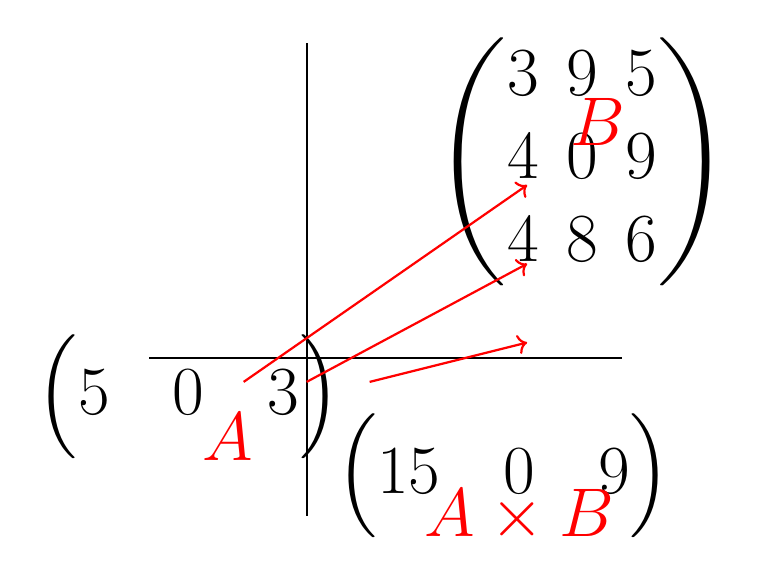
\begin{tikzpicture}
        % Axes
        \draw[thick] (-2,0) -- (4,0);
        \draw[thick] (0,-2) -- (0,4);
        
        % Ensembles A et B
        \node at (-1.5,-0.5) {\Huge $\Big( 5 \quad 0 \quad 3 \Big)$};
        \node at (3.5,2.5) {\Huge $\begin{pmatrix} 3 & 9 & 5 \\ 4 & 0 & 9 \\ 4 & 8 & 6 \end{pmatrix}$};
        
        % Produit Cartésien
        \node at (2.5,-1.5) {\Huge $\Big( 15 \quad 0 \quad 9 \Big)$};

        % Flèches rouges (associations)
        \draw[->, red, thick] (-0.8,-0.3) -- (2.8,2.2);
        \draw[->, red, thick] (0,-0.3) -- (2.8,1.2);
        \draw[->, red, thick] (0.8,-0.3) -- (2.8,0.2);

        % Labels
        \node[red] at (-1,-1) {\Huge $A$};
        \node[red] at (3.7,3) {\Huge $B$};
        \node[red] at (2.7,-2) {\Huge $A \times B$};

    \end{tikzpicture}
  \end{center}

  \centering{\includegraphics[width=0.7\textwidth]{images/matrices.png}}



  \raggedright XXXX

  \subsection{Inversion des M carrées}

  \begin{itemize}
    \item Soit $A\in M_n$ \\ A est inversible ssi $\exists A^{-1} \in M_n ~, ~~ A\times A^{-1} = A^{-1} \times A = I_n$
    \item Si A est inversible : 
    \begin{itemize}
      \item $A^{-1}$ est unique
      \item avec $A = \begin{bmatrix}
        a & b \\
        c & d 
      \end{bmatrix}
      \iff det(A) = ad - bc$ ~, $\boxed{A^{-1} = \frac{1}{det(A)}
        \begin{bmatrix}
          d & -b \\ 
          -c & a
        \end{bmatrix}}$
    \end{itemize}
  \end{itemize}








  \newpage


  \begin{center}

  \hfill
  \begin{verbatim}
    _  _    ___  _  _
    | || |  / _ \| || |
    | || |_| | | | || |_
    |__   _| |_| |__   _|
      |_|  \___/   |_|

                  _   _     
                  | | | |    
  _ __ ___   __ _| |_| |__   ____
  | '_ ` _ \ / _` | __| '_ \ / ___|
  | | | | | | (_| | |_| | | |\___ \
  |_| |_| |_|\__,_|\__|_| |_||____/
  \end{verbatim}

  \hfill
  \end{center}

\end{document}

  \newpage


  \section{Corrigé controle maths complémentaires}

  I.
  \begin{enumerate}
    \item 
    \begin{enumerate}
      \item $f(x)=1$ admet 2 solutions, \textbf{une sur $[-5;1]$ et une sur} [1;2]
      \item idem
      \item $f(x)=4$ n'admet pas de solution \textbf{sur} $[-10;5]$
    \end{enumerate}
    \item bien
  \end{enumerate}

  II.

  \begin{enumerate}
    \item 
    \begin{enumerate}
      \item 
    \end{enumerate}


  \end{enumerate}



